% !TeX program = pdflatex
% !TeX root = main.tex
% ==============================================================================
% Systematic Literature Review Manuscript (`M01_agentic_se_slr_20261111`)
% Exact 48-Month Window: 2022-11-01 to 2026-10-31 (N = 193 Primary Studies)
% ==============================================================================
\documentclass[10pt,twocolumn,a4paper]{article}

\usepackage[utf8]{inputenc}
\usepackage[T1]{fontenc}
\usepackage{lmodern}
\usepackage[margin=0.72in,top=0.8in,bottom=0.85in]{geometry}
\usepackage{amsmath,amssymb,amsfonts}
\usepackage{booktabs}
\usepackage{tabularx}
\usepackage{multirow}
\usepackage{array}
\usepackage{graphicx}
\usepackage{xcolor}
\usepackage{tikz}
\usetikzlibrary{shapes.geometric, arrows.meta, positioning, fit, calc, backgrounds}
\usepackage{microtype}
\usepackage{enumitem}
\usepackage{indentfirst}
\usepackage{xurl}
\usepackage{placeins}
\usepackage{hyperref}
\usepackage{cite}
\usepackage{caption}

\captionsetup{font=small,labelfont=bf,skip=4pt}
\setlength{\columnsep}{0.24in}
\setlength{\parindent}{1.5em}
\emergencystretch=1.5em
\raggedbottom

\setcounter{topnumber}{4}
\setcounter{bottomnumber}{4}
\setcounter{totalnumber}{8}
\setcounter{dbltopnumber}{4}
\renewcommand{\topfraction}{0.90}
\renewcommand{\bottomfraction}{0.85}
\renewcommand{\textfraction}{0.08}
\renewcommand{\floatpagefraction}{0.88}
\renewcommand{\dbltopfraction}{0.90}
\renewcommand{\dblfloatpagefraction}{0.88}
\setlength{\dblfloatsep}{8pt plus 2pt minus 2pt}
\setlength{\dbltextfloatsep}{10pt plus 2pt minus 2pt}
\setlength{\floatsep}{7pt plus 2pt minus 2pt}
\setlength{\textfloatsep}{9pt plus 2pt minus 2pt}
\setlength{\intextsep}{8pt plus 2pt minus 2pt}
\makeatletter
\setlength{\@fptop}{0pt}
\setlength{\@fpsep}{8pt}
\setlength{\@fpbot}{0pt plus 1fil}
\setlength{\@dblfptop}{0pt}
\setlength{\@dblfpsep}{8pt}
\setlength{\@dblfpbot}{0pt plus 1fil}
\renewcommand\section{\@startsection{section}{1}{\z@}{-2.8ex \@plus -0.6ex \@minus -0.2ex}{1.4ex \@plus 0.2ex}{\normalfont\Large\bfseries\raggedright}}
\renewcommand\subsection{\@startsection{subsection}{2}{\z@}{-2.2ex \@plus -0.5ex \@minus -0.2ex}{1.0ex \@plus 0.2ex}{\normalfont\large\bfseries\raggedright}}
\makeatother
\let\oldthebibliography\thebibliography
\renewcommand{\thebibliography}[1]{\oldthebibliography{#1}\setlength{\itemsep}{2pt plus 0.5pt minus 1pt}\setlength{\parskip}{0pt}}

\definecolor{navyblue}{RGB}{18, 53, 105}
\definecolor{slate}{RGB}{55, 71, 79}
\definecolor{tealaccent}{RGB}{0, 121, 107}
\definecolor{crimson}{RGB}{183, 28, 28}
\definecolor{amber}{RGB}{230, 81, 0}
\definecolor{softgray}{RGB}{245, 247, 250}

\hypersetup{
    colorlinks=true,
    linkcolor=navyblue,
    citecolor=tealaccent,
    urlcolor=navyblue
}

\title{\LARGE \textbf{The Productivity--Verification Paradox in Agentic Software Engineering: A Systematic Literature Review of Architectures, Verification Bottlenecks, and Governance}}

\author{
    \textbf{Feiran Liu}\\
    \small China National Association of Engineering Consultants (CNAEC), Beijing, China\\
    \small ORCID: \texttt{0000-0002-9678-1299} \quad|\quad \texttt{liufr@pku.edu.cn}
}

\date{November 2026}

\begin{document}
\maketitle

\begin{abstract}
Generative AI tools in software engineering (SE) have evolved from single-turn code completion into repository-level coding agents. While controlled trials on bounded tasks report notable coding speedups, repository-scale telemetry and benchmark studies point to a recurring \textbf{Productivity--Verification Paradox}: faster patch generation shifts bottlenecks into downstream review queues, exposes incomplete test suites, and increases human verification effort. Following PRISMA 2020 and Kitchenham's SE guidelines over the 48-month window from November 1, 2022 through October 31, 2026, we retrieved \textbf{6,121} records across OpenAlex, arXiv, Crossref, Semantic Scholar, and API-verified snowballing, screened \textbf{4,205} unique records, assessed \textbf{1,810} full-text reports under a four-criterion preprint screening protocol, and synthesized \textbf{193} primary studies (\textbf{155} peer-reviewed articles [80.3\%] and \textbf{38} moderated preprints [19.7\%]). We organize the corpus into a \textbf{Four-Layer Taxonomy}: (L1) Context \& Memory Management, (L2) Planning \& Orchestration Topology, (L3) Program Analysis \& Test Verification, and (L4) Socio-Technical \& Contract Governance. Across four research questions, synthesized studies indicate that: (1) enterprise autocomplete trials raise task throughput (+26.08\%), whereas published industrial studies report +105.9\% year-over-year diff-size growth and open-source pull-request (PR) studies report human edits on 45.1\% of merged agent PRs ($n=567$), 2.66\% post-merge reverts (no matched human baseline), and $3.5\times$ merge delays on inconsistent PRs; (2) test-suite studies identify 32.67\% SWE-bench solution leakage, 31.08\% weak-test passes, and 29.6\% behavioral patch divergence; (3) AST/PDG search, SMT dataflow, and bounded model checking lift verified Rust transpilation from 1\% to 42\%; and (4) graph localization ($\sim$86\% localization cost cut), context distillation (51.8\%--71.3\% token reduction), early termination (19\%--55\% total cost cut), and delegation guards bound inference cost and Model Context Protocol (MCP) security risks.
\end{abstract}

\vspace{0.4em}
\noindent\textbf{Keywords:} Agentic Software Engineering, Coding Agents, Automated Code Review, Mutation Testing, Program Analysis Grounding, Context Retrieval Economics, Model Context Protocol, Systematic Literature Review, PRISMA 2020.

\section{Introduction}
\label{sec:intro}

Between November 1, 2022 and October 31, 2026, generative AI tools in software engineering (SE) evolved from inline code completion into repository-level coding agents. Early deployments of pre-trained code models such as Codex~\cite{chen2021evaluating} and GitHub Copilot~\cite{vaithilingam2022expectation,dakhel2023github,ziegler2024measuring} worked mainly as single-turn autocomplete assistants inside integrated development environments (IDEs). Controlled lab studies on bounded programming tasks reported 55.8\% faster task completion~\cite{peng2023impact}, and field randomized controlled trials (RCTs) across Microsoft, Accenture, and an anonymous Fortune 100 company ($N=4,867$ developers) measured a 26.08\% increase in completed tasks~\cite{cui2026effects}. Over the subsequent four years, research and industrial tooling expanded from token-level suggestions to \emph{repository-level autonomous coding agents} that plan multi-step edits, invoke shell tools, traverse multi-file dependency graphs, run test suites, and open pull requests (PRs)~\cite{jimenez2024swebench,yang2024sweagent,wang2025openhands,li2026aidev}.

Grouping our $N=193$ primary studies by first public release date (\texttt{first\_release\_date}) into four 12-month cohorts---so that publication indexing lags do not distort timing---illustrates how focus shifted year by year: \textbf{Cohort Y1} (\texttt{2022-11}--\texttt{2023-10}, $n=22$, 11.4\%) introduced closed-loop tool invocation, verbal self-reflection, and hybrid test generation~\cite{yao2023react,schick2023toolformer,shinn2023reflexion,lemieux2023codamosa}; \textbf{Cohort Y2} (\texttt{2023-11}--\texttt{2024-10}, $n=33$, 17.1\%) established repository benchmarks (\texttt{SWE-bench}), Agent--Computer Interfaces (ACIs), structured repair pipelines, and multi-agent workflows~\cite{jimenez2024swebench,yang2024sweagent,xia2024demystifying,hong2024metagpt,qian2024chatdev}; \textbf{Cohort Y3} (\texttt{2024-11}--\texttt{2025-10}, $n=46$, 23.8\%) examined benchmark leakage, patch overfitting, and task slowdowns in mature open-source codebases~\cite{yu2025utboost,wang2025solved,rondon2025evaluating,watanabe2025use,becker2025measuring}; and \textbf{Cohort Y4} (\texttt{2025-11}--\texttt{2026-10}, $n=92$, 47.7\%) studied ecosystem-scale agentic PR volume, review-queue delays, Model Context Protocol (MCP) security risks, and risk-tiered governance~\cite{li2026aidev,adams2026automating,gong2026analyzing,oukhay2026code,chowdhury2026industry,arora2026specifying}. Cross-walk counts by publication year are reported in Section~\ref{sec:methodology}.3.

Taken together, these studies point to a recurring tension that we term the \textbf{Productivity--Verification Paradox}: \emph{when upstream patch generation accelerates faster than execution-grounded verification and review capacity, the primary bottleneck in software delivery shifts from writing code to reviewing changes, checking behavioral correctness, and maintaining merged code}. In industrial telemetry reported at Meta by Adams et al.~\cite{adams2026automating}, significant lines of code per human-landed diff were found to grow by 105.9\% year over year and per-developer diff volume by 51\%---with over 80\% of that growth attributed by the authors to agentic AI---widening the gap between code output and human review bandwidth. In open-source ecosystems, large-scale mining of 932,791 agent-authored PRs~\cite{li2026aidev}, empirical studies of review effort, message--code mismatch, and post-merge reverts~\cite{watanabe2025use,gong2026analyzing,ehsani2026where,oukhay2026code,chowdhury2026industry,milanese2026humanagent}, and an OSS maintainer RCT~\cite{becker2025measuring} likewise suggest that unverified diff volume lengthens review queues, contributes to post-merge reverts from unintended side effects, and allows subtle regressions to pass incomplete test suites~\cite{aleithan2026swebench,wang2025solved}.

Foundational reviews have established an essential baseline for this rapidly evolving area. In software engineering, Fan et al.~\cite{fan2023large} outlined an early research roadmap for large language models across SE tasks, and Hou et al.~\cite{hou2024large} conducted a comprehensive systematic review of 395 research articles from January 2017 to January 2024, thoroughly charting code generation, summarization, and comprehension prior to the emergence of repository-level coding agents. In parallel, seminal surveys by Xi et al.~\cite{xi2023rise} and Wang et al.~\cite{wang2024survey} synthesized general-purpose LLM agent planning, memory, and tool-use architectures across broader AI domains. Because repository-scale coding agents, benchmark test-oracle audits, Model Context Protocol (MCP) tool security, and large-scale agentic PR telemetry largely matured between 2024 and 2026, a focused synthesis of these recent SE-specific developments serves as a timely continuation of those earlier reviews. Building on that foundational literature, this study seeks to complement existing work in three main respects:
\begin{enumerate}[leftmargin=*,nosep]
    \item \textbf{POMDP \& Analytical Queueing Conceptual Lens:} A two-level analytical framework connecting trajectory-level POMDP belief drift and specification gaming with organization-level Amdahl cycle-time bounds~\cite{amdahl1967validity} and heavy-traffic $G/G/k$ review queueing~\cite{kingman1961single,sakasegawa1977approximation}.
    \item \textbf{Four-Layer Taxonomy \& Verbatim-Verified PRISMA 2020 Synthesis ($N=193$):} A reproducible 48-month multi-database synthesis (155 peer-reviewed articles [80.3\%] and 38 moderated preprints [19.7\%]) structured as an orthogonal \texttt{L1}--\texttt{L4} $\times$ \texttt{RQ1}--\texttt{RQ4} classification, supported by a 38-claim abstract-verified ledger, a 5-criterion Risk-of-Bias rubric, and a publication-stage sensitivity check.
    \item \textbf{Benchmark Comparison \& Governance Roadmap:} A structured comparison of 16 representative benchmark and telemetry suites across reset assumptions, test-oracle design, and inference cost, distilled into seven research directions (\texttt{C1}--\texttt{C7}) for dependable agentic SE.
\end{enumerate}

\section{Background and Analytical Framework}
\label{sec:background}

\begin{table*}[t!]
\centering
\caption{Complete Summary of Mathematical Notation, POMDP Seven-Tuple Elements, and Analytical Queueing Variables (Sections~\ref{sec:background}.1--\ref{sec:background}.2).}
\label{tab:notation}
\scriptsize
\setlength{\tabcolsep}{4.0pt}
\renewcommand{\arraystretch}{0.98}
\begin{tabularx}{\textwidth}{>{\raggedright\arraybackslash}p{4.12cm} X}
\toprule
\textbf{Symbol / Function} & \textbf{Formal Domain \& Software Engineering Interpretation} \\
\midrule
\multicolumn{2}{l}{\textbf{(A) Repository-Level Closed-Loop POMDP Formulation (Section~\ref{sec:background}.1, Eqs.~\eqref{eq:pomdp}--\eqref{eq:policy})}} \\
$p_\theta(y \mid x)$ & Stateless single-turn code-completion mapping generating token sequence $y$ from prompt $x$ under model weights $\theta$. \\
$\mathcal{M} = \langle \mathcal{S}, \mathcal{A}, \mathcal{O}, \mathcal{T}, \Omega, R, \gamma \rangle$ & Seven-tuple Partially Observable Markov Decision Process governing multi-step agent--repository interaction over $t \in \{0,1,\dots\}$. \\
$\mathcal{S}$ ($s, s' \in \mathcal{S}$) & Latent full repository state space (source tree, build/container state, dependency graph, tests, unwritten intent; $s$ at $t-1$, $s'$ at $t$). \\
$\mathcal{A}$ ($a_t \in \mathcal{A}$) & Agent action space comprising file edits/patches, AST/regex search, shell commands, test execution, and MCP tool invocations. \\
$\mathcal{O}$ ($o_t \in \mathcal{O}$) & Partial observation space returned via the Agent--Computer Interface (ACI): truncated stdout/stderr logs, compiler diagnostics, and code slices. \\
$\mathcal{T}(s' \mid s, a_{t-1})$ & State-transition probability kernel defining the probability of moving from latent state $s$ to $s'$ after executing action $a_{t-1}$. \\
$\Omega(o_t \mid s', a_{t-1})$ & Observation-emission probability function defining the probability of receiving ACI output $o_t$ upon reaching state $s'$ via $a_{t-1}$. \\
$R(s,a),\; R^\star(s_t),\; \widehat{R}(s_t),\; T_{\text{existing}}$ & Step reward function $R$; true specification-satisfaction reward $R^\star(s_t)$ vs.\ empirical proxy $\widehat{R}(s_t)$ evaluated on incomplete existing tests $T_{\text{existing}}$. \\
$\gamma \in [0, 1)$ & Temporal discount factor trading off immediate single-issue test passage against multi-commit architectural maintainability. \\
$b_t(s'),\; h_t,\; \mathcal{C}(\cdot),\; \widehat{b}_t = \mathcal{C}(h_t)$ & Exact Bayesian posterior belief $b_t(s')$ over $\mathcal{S}$, full trajectory $h_t = (o_0, a_0, \dots, a_{t-1}, o_t)$, context-compaction operator $\mathcal{C}$, and compacted state $\widehat{b}_t$. \\
$\pi_\theta(a_t \mid \widehat{b}_t)$ & Parameterized stochastic agent policy sampling action $a_t \in \mathcal{A}$ conditioned on compacted context representation $\widehat{b}_t$. \\
\midrule
\multicolumn{2}{l}{\textbf{(B) Cycle-Time Decomposition \& Analytical $G/G/k$ Review Queueing Lens (Section~\ref{sec:background}.2, Eq.~\eqref{eq:kingman})}} \\
$T_0,\; T_{\text{lead}}(\alpha),\; f_c \in (0,1)$ & Baseline end-to-end delivery lead time $T_0$, realized lead time $T_{\text{lead}}(\alpha)$ under coding speedup $\alpha$, and active coding share $f_c$ of $T_0$. \\
$\alpha \ge 1,\; \lambda(\alpha) > 0$ & Task-level active coding throughput multiplier $\alpha$ and the induced pull-request (PR) arrival rate $\lambda(\alpha)$ entering human review. \\
$G/G/k,\; k \in \mathbb{Z}^+$ & Kendall queueing notation: general ($G$) PR inter-arrival distribution, general ($G$) review service-time distribution, and $k$ parallel human reviewers. \\
$\sigma \ge 0,\; \mu(\sigma) > 0$ & Patch size/cross-module dispersion $\sigma$ and per-reviewer service rate $\mu(\sigma)$ (decreasing with $\sigma$; mean review service time $1/\mu(\sigma)$). \\
$\rho = \lambda(\alpha) / [k\,\mu(\sigma)] \in [0, 1)$ & Reviewer server utilization (traffic intensity; steady-state queue stability requires $\rho < 1$). \\
$c_a^2,\; c_s^2 \ge 0,\; E[W_q]$ & Squared coefficients of variation ($\text{Var}/\text{Mean}^2$) of PR inter-arrival ($c_a^2$) and review service times ($c_s^2$), and expected queue wait time $E[W_q]$. \\
\bottomrule
\end{tabularx}
\end{table*}

\subsection{Closed-Loop Agentic SE as a Repository POMDP}
Whereas single-turn code completion models a stateless mapping $p_\theta(y \mid x)$ from prompt tokens $x$ to a code snippet $y$ under parameters $\theta$, a repository-level coding agent interacts repeatedly with its development environment across steps $t \in \{0, 1, \dots\}$. This closed loop can be represented as a seven-tuple Partially Observable Markov Decision Process (POMDP)~\cite{kaelbling1998planning} $\mathcal{M} = \langle \mathcal{S}, \mathcal{A}, \mathcal{O}, \mathcal{T}, \Omega, R, \gamma \rangle$ (summarized in Table~\ref{tab:notation}). Here $\mathcal{S}$ is the latent repository state space (source files, build/container state, cross-module dependencies, test suite, and unwritten design intent), with $s \in \mathcal{S}$ at step $t-1$ and $s' \in \mathcal{S}$ at step $t$; $\mathcal{A}$ is the action space ($a_t \in \mathcal{A}$: file edits, AST/grep searches, shell commands, test runs, and MCP tool calls); and $\mathcal{O}$ is the partial observation space ($o_t \in \mathcal{O}$: truncated stdout/stderr logs, compiler diagnostics, and code snippets returned via an Agent--Computer Interface~\cite{yang2024sweagent,wang2025openhands}). State evolution follows the transition kernel $\mathcal{T}(s' \mid s, a_{t-1})$ and observation function $\Omega(o_t \mid s', a_{t-1})$, while $R(s, a)$ denotes the step specification-satisfaction reward discounted by $\gamma \in [0, 1)$ over multi-step maintenance. Exact Bayesian updating of the posterior belief $b_t(s')$ over latent states takes the form:
\begin{equation}
\label{eq:pomdp}
b_t(s') \propto \Omega(o_t \mid s', a_{t-1}) \sum_{s \in \mathcal{S}} \mathcal{T}(s' \mid s, a_{t-1})\, b_{t-1}(s).
\end{equation}

Because $\mathcal{S}$ cannot be enumerated in real codebases, practical LLM agents apply a bounded context-compaction operator $\mathcal{C}(\cdot)$ to the interaction history $h_t = (o_0, a_0, \dots, a_{t-1}, o_t)$ to form an approximate context state $\widehat{b}_t = \mathcal{C}(h_t)$, and draw actions $a_t$ from a stochastic policy $\pi_\theta$:
\begin{equation}
\label{eq:policy}
a_t \sim \pi_\theta\!\left(\cdot \mid \widehat{b}_t\right), \qquad \widehat{b}_t = \mathcal{C}(h_t).
\end{equation}

Equations~\eqref{eq:pomdp}--\eqref{eq:policy} highlight two recurring failure modes. First, as $h_t$ grows during multi-file exploration, reduced recall in middle context positions~\cite{liu2024lost} and lossy context paging~\cite{packer2023memgpt} widen the gap between $\widehat{b}_t$ and $b_t$ (\emph{belief drift}), compounding errors across sequential maintenance tasks~\cite{jin2026chainswe}. Second, when the empirical reward signal $\widehat{R}(s_t)$ relies solely on an incomplete regression suite $T_{\text{existing}}$ rather than full specification satisfaction $R^\star(s_t)$, optimization favors \emph{specification gaming} and plausible-but-incorrect patches~\cite{aleithan2026swebench,yu2025utboost,wang2025solved}, including modifying failing assertions when test files are writable in \texttt{ImpossibleBench}~\cite{zhong2025impossiblebench}.

\subsection{Cycle-Time Decomposition and Analytical Queueing Lens}
To link individual coding speedups with team-level delivery times, we pair Amdahl's law with a standard queueing formulation. Because primary studies do not yet report uniform second-moment PR arrival and review-time logs, Eqs.~\eqref{eq:pomdp}--\eqref{eq:kingman} serve as an analytical framework for organizing empirical hypotheses rather than as structurally fitted equations. Let $T_0$ denote baseline end-to-end lead time and $f_c \in (0,1)$ the fraction spent in active code writing. By Amdahl's law~\cite{amdahl1967validity}, speeding up coding by a factor $\alpha \ge 1$ bounds friction-free lead time at $T_{\text{lead}}^{\min}(\alpha) = T_0(1 - f_c + f_c/\alpha)$, capping overall speedup at $(1 - f_c + f_c/\alpha)^{-1}$. In pull-based development, however, higher coding output also raises the PR arrival rate $\lambda(\alpha)$ into a $G/G/k$ review queue with general ($G$) inter-arrival and review-service distributions across $k$ human reviewers. Each reviewer processes changes at rate $\mu(\sigma)$ (mean review time $1/\mu(\sigma)$), which slows as diff size and cross-module spread $\sigma$ increase~\cite{adams2026automating,oukhay2026code}. Under Kingman's heavy-traffic approximation~\cite{kingman1961single} and Sakasegawa's $G/G/k$ extension~\cite{sakasegawa1977approximation}, expected review queue wait time $E[W_q]$ is approximated by:
\begin{equation}
\label{eq:kingman}
\begin{aligned}
E[W_q] &\approx \left(\frac{c_a^2 + c_s^2}{2}\right) \frac{\rho^{\sqrt{2(k+1)}-1}}{k(1-\rho)} \cdot \frac{1}{\mu(\sigma)}, \\
\rho &= \frac{\lambda(\alpha)}{k\,\mu(\sigma)} < 1,
\end{aligned}
\end{equation}
where $\rho \in [0, 1)$ is reviewer server utilization and $c_a^2, c_s^2 \ge 0$ denote the squared coefficients of variation ($\text{Var}/\text{Mean}^2$) of PR inter-arrival and review-service times (Table~\ref{tab:notation}).

Equation~\eqref{eq:kingman} explains why faster code authoring does not automatically yield faster merges: when coding agents raise the arrival rate $\lambda(\alpha)$, enlarge diff sizes (reported at +105.9\% YoY in~\cite{adams2026automating}), and increase review-effort variance $c_s^2$ through message--code mismatches or code redundancy and technical debt~\cite{gong2026analyzing,huang2026more}, reviewer utilization $\rho$ approaches 1 and $E[W_q] \propto (1-\rho)^{-1}$ rises steeply, increasing end-to-end lead time $T_{\text{lead}}(\alpha) = T_{\text{lead}}^{\min}(\alpha) + E[W_q]$.

\section{Systematic Review Methodology}
\label{sec:methodology}

This review follows Kitchenham and Charters' SE systematic review guidelines and subsequent updates~\cite{kitchenham2007guidelines,kitchenham2009systematic,kitchenham2015evidence} together with the PRISMA 2020 statement~\cite{page2021prisma} (27-item mapping in Appendix~\ref{app:prisma}). Before running the November 11, 2026 harvest, we froze the protocol locally in \texttt{00\_protocol.md}. Because the protocol was not deposited in an external registry such as PROSPERO or OSF, we note this limitation in Section~\ref{sec:threats} and provide SHA-256-checksummed raw API payloads alongside deterministic screening scripts.

\begin{table*}[t!]
\centering
\caption{Research Questions (RQs), Deterministic Sub-Layer Mapping, Mutually Exclusive Primary Partition ($N=193$), and Multi-Label Coverage.}
\label{tab:rqs}
\footnotesize
\setlength{\tabcolsep}{4.0pt}
\begin{tabularx}{\textwidth}{l >{\raggedright\arraybackslash}p{2.20cm} >{\raggedright\arraybackslash}p{2.10cm} c c X}
\toprule
\textbf{ID} & \textbf{Core Dimension} & \textbf{Primary Sub-Layers} & \textbf{Primary $n$} & \textbf{Multi-Tag $n$} & \textbf{Analytical Question \& Operational Metrics} \\
\midrule
\textbf{RQ1} & Delivery \& Topologies & \texttt{L2.1--L2.3, L4.2} & 66 & 111 & How do single-/multi-agent architectures reshape task velocity, PR merge latency, revert rates, and reviewer queue utilization? \\
\textbf{RQ2} & Verification \& Review & \texttt{L3.2--L3.3} & 55 & 94 & Why do automated test-generation and code-review agents exhibit gaps between syntactic pass rates, mutation kills, and semantic correctness? \\
\textbf{RQ3} & Program Grounding & \texttt{L3.1} & 15 & 108 & To what extent do AST/PDG analysis, dataflow facts, and formal model checking mitigate hallucinated patches and unsafe translations? \\
\textbf{RQ4} & Economics \& Governance & \texttt{L1.1--L1.3, L4.1, L4.3} & 57 & 103 & Which context-compression schemes, prompt-injection/MCP defenses, and declarative requirement contracts bound cost and security risk? \\
\midrule
\textbf{Total} & \textbf{Exact Partition} & \textbf{All 12 Sub-Layers} & \textbf{193} & \textbf{---} & \textbf{Mutually exclusive primary partition ($66+55+15+57=193$); cross-layer evidence tracked via multi-label \texttt{rqs}.} \\
\bottomrule
\end{tabularx}
\end{table*}

\subsection{Research Questions and Search Strategy}
Table~\ref{tab:rqs} defines our four Research Questions (\texttt{RQ1}--\texttt{RQ4}), spanning agentic delivery velocity and orchestration topologies (\texttt{RQ1}), automated test and code-review verification bottlenecks (\texttt{RQ2}), static/dynamic program-analysis grounding (\texttt{RQ3}), and context economics, tool security, and contract governance (\texttt{RQ4}).

To eliminate partial-month truncation while covering an exact four-year period since the emergence of modern chat- and agent-based SE workflows, we fixed the publication/release window to \texttt{2022-11-01} through \texttt{2026-10-31} (exact 48 months). We executed live programmatic queries across four bibliographic databases plus API-verified citation snowballing (100\% verbatim query strings in Appendix~\ref{app:queries}):
\begin{itemize}[leftmargin=*,nosep]
    \item \textbf{OpenAlex Works API:} Three-block conjunctive Boolean query across title/abstract fields (\textbf{1,323} records across 7 pages).
    \item \textbf{arXiv Export API:} Field-scoped query across \texttt{cs.SE}, \texttt{cs.AI}, \texttt{cs.CL}, \texttt{cs.PL}, and \texttt{cs.CR} (\textbf{2,224} records across 8 pages).
    \item \textbf{Crossref REST API:} Six targeted journal/proceedings bibliographic sub-queries (\textbf{1,200} records).
    \item \textbf{Semantic Scholar Bulk Graph API:} Conjunctive Computer Science full-window query (\textbf{1,299} records).
    \item \textbf{Citation Snowballing (PRISMA ``Other Methods''):} Backward and forward tracking from landmark SE agent benchmarks and field studies, verified individually via official OpenAlex/Crossref/arXiv APIs (\textbf{75} records).
\end{itemize}

\begin{table}[t!]
\centering
\caption{Inclusion Criteria (IC1--IC4) and Exclusion Criteria (EC1--EC6).}
\label{tab:criteria}
\footnotesize
\setlength{\tabcolsep}{3.8pt}
\begin{tabularx}{\columnwidth}{l X}
\toprule
\textbf{Code} & \textbf{Operational Criterion} \\
\midrule
\textbf{IC1} & \textbf{IC1-A}: Closed-loop LLM SE agent interacting with tools, sandboxes, or repositories; \emph{or} \textbf{IC1-B}: Empirical RCT, MSR study, queueing analysis, or security/governance audit of AI coding workflows. \\
\textbf{IC2} & Reports original quantitative benchmarks, field/repository telemetry, or formal verification experiments. \\
\textbf{IC3} & Peer-reviewed journal/conference article, \emph{or} moderated academic preprint meeting all 4 criteria (\textbf{G1}: complete manuscript with named authors on a moderated preprint server; \textbf{G2}: $\ge$6 pages; \textbf{G3}: verifiable benchmark/open artifact; \textbf{G4}: citations $\ge$90 [$\le$2024], $\ge$45 [2025], or $\ge$18 [2026]). \\
\textbf{IC4} & English manuscript first released or published within \texttt{2022-11-01} to \texttt{2026-10-31} (48 months). \\
\midrule
\textbf{EC1} & Off-domain non-SE application (medicine, robotics, chemistry, blockchain/DeFi, K--12 pedagogy, 3D gaming), non-English, or outside window. \\
\textbf{EC2} & Single-turn static token completion or NLP classification (e.g., comment sentiment) without closed-loop interaction or workflow telemetry. \\
\textbf{EC3} & Secondary/non-empirical literature (surveys, SLRs, position papers, enterprise whitepapers, preregistrations, $<4$-page or anonymous stubs). \\
\textbf{EC4} & Insufficient SE repository/verification grounding or unexecuted evaluation proposals. \\
\textbf{EC5} & Preprints not yet meeting all four criteria (\textbf{G1--G4}) of the \textbf{IC3} screening protocol or broad-scope low-selectivity venues. \\
\textbf{EC6} & Companion replication packages, standalone data/code archives, or earlier preprints consolidated into their published journal/proceedings version. \\
\bottomrule
\end{tabularx}
\end{table}
% --- FIGURE 1: PRISMA 2020 THREE-STAGE FLOW DIAGRAM ---
\begin{figure*}[t!]
\centering
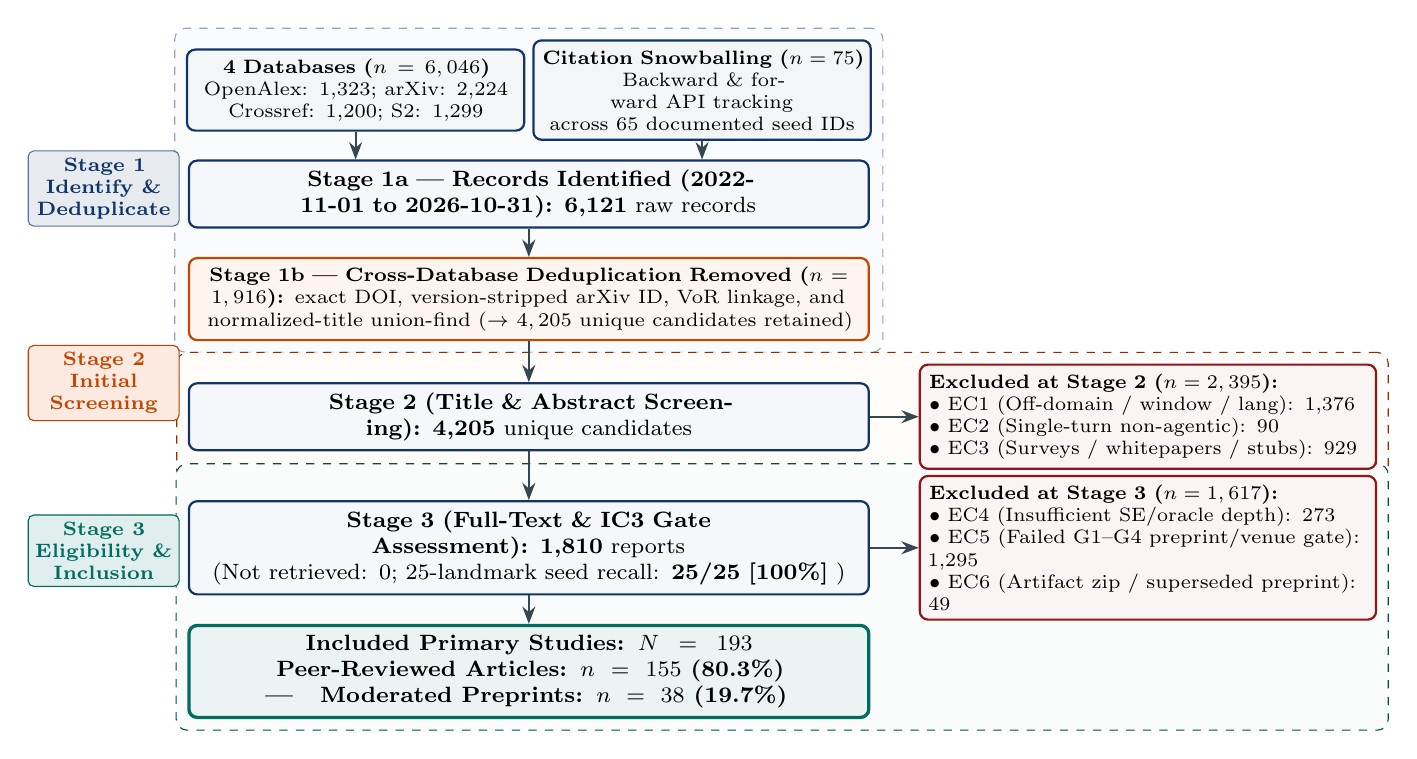
\begin{tikzpicture}[
    node distance=0.36cm and 0.62cm,
    srcbox/.style={rectangle, rounded corners=3pt, draw=navyblue, thick, fill=navyblue!5, text width=4.05cm, minimum height=0.84cm, align=center, font=\scriptsize},
    box/.style={rectangle, rounded corners=3pt, draw=navyblue, thick, fill=softgray, text width=8.40cm, minimum height=0.72cm, align=center, font=\footnotesize},
    dupbox/.style={rectangle, rounded corners=3pt, draw=amber!85!black, thick, fill=amber!6, text width=8.40cm, minimum height=0.70cm, align=center, font=\scriptsize},
    sidebox/.style={rectangle, rounded corners=3pt, draw=crimson!80!black, thick, fill=crimson!5, text width=5.56cm, minimum height=0.76cm, align=left, font=\scriptsize},
    incbox/.style={rectangle, rounded corners=3pt, draw=tealaccent!90!black, very thick, fill=tealaccent!8, text width=8.40cm, minimum height=0.84cm, align=center, font=\footnotesize\bfseries},
    stgbadge/.style={rectangle, rounded corners=2pt, text width=1.74cm, align=center, font=\scriptsize\bfseries, inner sep=2.5pt},
    arr/.style={-{Stealth[length=2.2mm]}, thick, draw=slate}
]
\node[srcbox] (db) at (-2.20, 0) {\textbf{4 Databases ($n = 6,046$)}\\
OpenAlex: 1,323; arXiv: 2,224\\
Crossref: 1,200; S2: 1,299};
\node[srcbox] (sb) at (2.20, 0) {\textbf{Citation Snowballing ($n = 75$)}\\
Backward \& forward API tracking\\
across 65 documented seed IDs};

\node[box] (id) at (0, -1.32) {\textbf{Stage 1a --- Records Identified (2022-11-01 to 2026-10-31):} \textbf{6,121} raw records};

\node[dupbox, below=of id] (dup) {\textbf{Stage 1b --- Cross-Database Deduplication Removed ($n = 1,916$):} exact DOI, version-stripped arXiv ID, VoR linkage, and normalized-title union-find ($\to 4,205$ unique candidates retained)};

\node[box, below=0.52cm of dup] (scr) {\textbf{Stage 2 (Title \& Abstract Screening):} \textbf{4,205} unique candidates};

\node[sidebox, right=of scr] (ex2) {\textbf{Excluded at Stage 2 ($n = 2,395$):}\\
$\bullet$ EC1 (Off-domain / window / lang): 1,376\\
$\bullet$ EC2 (Single-turn non-agentic): 90\\
$\bullet$ EC3 (Surveys / whitepapers / stubs): 929};

\node[box, below=0.62cm of scr] (elig) {\textbf{Stage 3 (Full-Text \& IC3 Gate Assessment):} \textbf{1,810} reports\\
(Not retrieved: 0; 25-landmark seed recall: \textbf{25/25 [100\%]} )};

\node[sidebox, right=of elig] (ex3) {\textbf{Excluded at Stage 3 ($n = 1,617$):}\\
$\bullet$ EC4 (Insufficient SE/oracle depth): 273\\
$\bullet$ EC5 (Failed G1--G4 preprint/venue gate): 1,295\\
$\bullet$ EC6 (Artifact zip / superseded preprint): 49};

\node[incbox, below=of elig] (inc) {Included Primary Studies: $N = 193$\\
Peer-Reviewed Articles: $n = 155$ (80.3\%) \quad|\quad Moderated Preprints: $n = 38$ (19.7\%)};

\node[stgbadge, draw=navyblue!70, fill=navyblue!10, text=navyblue] at (-5.40, -1.25) {Stage 1\\Identify \&\\Deduplicate};
\node[stgbadge, draw=amber!80!black, fill=amber!12, text=amber!85!black] at (-5.40, -3.72) {Stage 2\\Initial\\Screening};
\node[stgbadge, draw=tealaccent!85!black, fill=tealaccent!12, text=tealaccent!90!black] at (-5.40, -5.85) {Stage 3\\Eligibility \&\\Inclusion};

\begin{scope}[on background layer]
\node[draw=navyblue!45, dashed, rounded corners=4pt, fill=navyblue!2, inner sep=4pt, fit=(db)(sb)(id)(dup)] {};
\node[draw=amber!60!black, dashed, rounded corners=4pt, fill=amber!2, inner sep=4pt, fit=(scr)(ex2)] {};
\node[draw=tealaccent!65!black, dashed, rounded corners=4pt, fill=tealaccent!2, inner sep=4pt, fit=(elig)(ex3)(inc)] {};
\end{scope}

\draw[arr] (db.south) -- (db.south |- id.north);
\draw[arr] (sb.south) -- (sb.south |- id.north);
\draw[arr] (id) -- (dup);
\draw[arr] (dup) -- (scr);
\draw[arr] (scr) -- (ex2);
\draw[arr] (scr) -- (elig);
\draw[arr] (elig) -- (ex3);
\draw[arr] (elig) -- (inc);
\end{tikzpicture}
\caption{PRISMA 2020 Three-Stage Funnel: Stage 1 Multi-Source Identification \& Union-Find Deduplication (\texttt{DB+SB $\to$ ID $\to$ DUP}), Stage 2 Title/Abstract Screening, and Stage 3 Full-Text \& 4-Point Preprint Gate Assessment ($N = 193$ primary studies across \texttt{2022-11-01} to \texttt{2026-10-31}; counts derived programmatically from \texttt{02\_\allowbreak screening/\allowbreak screening\_\allowbreak log.\allowbreak csv}).}
\label{fig:prisma}
\end{figure*}

\subsection{Three-Stage Selection Funnel and Preprint Quality Gate}
Figure~\ref{fig:prisma} and Table~\ref{tab:criteria} detail our three-stage selection funnel across \texttt{02\_\allowbreak screening/\allowbreak screening\_\allowbreak log.\allowbreak csv}.

At \textbf{Stage 1 (Multi-Source Identification \& Cross-Database Deduplication)}, programmatic harvesting retrieved \textbf{6,046} database records and \textbf{75} API-verified snowball records, totaling \textbf{6,121} raw records. Union-find deduplication across normalized DOIs, version-stripped arXiv identifiers, OpenAlex Version-of-Record (VoR) links, and normalized titles removed \textbf{1,916} duplicates, retaining \textbf{4,205} unique candidates for screening.

At \textbf{Stage 2 (Title \& Abstract Screening)}, \textbf{2,395} records were excluded: \texttt{EC1} ($n=1,376$) removed off-domain topics and out-of-window items; \texttt{EC2} ($n=90$) removed single-turn non-agentic tasks lacking workflow telemetry; and \texttt{EC3} ($n=929$) removed secondary reviews, position papers, whitepapers, preregistration stubs, and non-English items (\texttt{IC4}).

At \textbf{Stage 3 (Full-Text \& Preprint Screening Assessment)}, all \textbf{1,810} remaining reports were assessed with \texttt{0} unretrieved reports. Peer-reviewed eligibility (\texttt{IC3}) encompassed 150 flagship SE, PL, security, ML, and management main-track articles plus 5 formally refereed companion/workshop papers~\cite{alshahwan2024automated,bouzenia2024repairagent,shetty2025syzygy,kanvar2026meets,feng2026sage} (full track inventory in Appendix~\ref{app:rubric}). Because rapid advances in agentic SE frequently appear on moderated academic preprint repositories ahead of journal or conference publication cycles, non-peer-reviewed Stage 3 candidates ($n=1,300$) were evaluated uniformly under a four-criterion screening protocol (\texttt{03\_\allowbreak extraction/\allowbreak preprint\_\allowbreak quality\_\allowbreak gate\_\allowbreak audit.\allowbreak csv}): \textbf{G1} complete research manuscript with named authorship hosted on a moderated academic preprint repository; \textbf{G2} full technical report of at least 6 pages; \textbf{G3} public benchmark, dataset, or open-source artifact; and \textbf{G4} age-stratified citation thresholds as of 2026-11-11 ($\ge 90$ for $\le 2024$, $\ge 45$ for 2025, $\ge 18$ for 2026, applied identically to database and snowballed candidates). Stage 3 excluded \textbf{1,617} reports under \texttt{EC4} ($n=273$, insufficient SE verification depth), \texttt{EC5} ($n=1,295$, including 1,262 preprints not yet meeting \texttt{G1}--\texttt{G4}), and \texttt{EC6} ($n=49$, standalone data/code archives or earlier preprints consolidated into their published versions).

Because this SLR was conducted by a single author, two-rater Cohen's $\kappa$~\cite{cohen1960coefficient,landis1977measurement} does not apply; instead, we encoded deterministic rule-based screening in \texttt{stage2\_\allowbreak and\_\allowbreak 3\_\allowbreak prisma.\allowbreak py} and verified \textbf{25/25 (100.0\%)} non-circular recall against landmark peer-reviewed seeds. A 12-day blind intra-rater re-screening and re-coding check (\texttt{2026-11-11} vs.\ \texttt{2026-11-23}, logged in \texttt{02\_\allowbreak screening/\allowbreak intra\_\allowbreak rater\_\allowbreak blind\_\allowbreak check\_\allowbreak n20.\allowbreak csv}) on a stratified 10\% ($n=20$) Stage 3 sample achieved \textbf{20/20 (100.0\%)} agreement on inclusion and \texttt{primary\_rq}, and \textbf{19/20 (95.0\%)} on secondary \texttt{rqs}, with the single borderline case \texttt{S106}~\cite{guo2026eet} documented in Appendix~\ref{app:rubric}.

\subsection{Data Extraction, Risk-of-Bias Rubric, and Synthesis Method}
For all $N=193$ included studies, automated scripts extracted bibliographic metadata, initial release dates (\texttt{first\_release\_date}, defining cohorts \texttt{Y1}--\texttt{Y4}), taxonomy sub-layers (\texttt{L1.1}--\texttt{L4.3}), mutually exclusive primary \texttt{RQ} (\texttt{primary\_rq}), and sorted multi-label \texttt{RQ} tags (\texttt{rqs}) into \texttt{03\_\allowbreak extraction/\allowbreak review\_\allowbreak matrix.\allowbreak csv}. By API-indexed publication year \texttt{year}, the corpus spans 2023 ($n=14$), 2024 ($n=36$), 2025 ($n=53$), and 2026 ($n=90$); reassigning 20 cross-year online-first articles~\cite{dong2023selfcollaboration,asare2023usercentered,yang2023whitefox,ma2024alibaba,yuan2024transagent,lin2024soen101,bouzenia2024repairagent,huang2024unidebugger,yang2024vert,xia2024demystifying,jia2024task,xu2025hallucination,guo2025swe,wang2025solved,ceka2025understanding,mu2025experepair,watanabe2025use,peng2025sweqa,oueslati2025refagent,horikawa2025agentic} to their subsequent archival volume years yields 11, 31, 51, and 100 studies, respectively. Secondary multi-label \texttt{rqs} were assigned only when a study reported quantitative metrics on the secondary \texttt{RQ}'s dependent variable or dedicated a standalone section or table to that mechanism. All 38 headline quantitative claims in \texttt{03\_\allowbreak extraction/\allowbreak verified\_\allowbreak evidence\_\allowbreak ledger.\allowbreak csv} passed automated assertions for contiguous verbatim abstract substrings and 100\% numeric-token coverage (exact regex normalization rules in Appendix~\ref{app:rubric}). Each study was also scored from 0--10 across a 5-criterion Quality \& Risk-of-Bias (RoB) rubric adapted from Kitchenham and Charters~\cite{kitchenham2007guidelines,kitchenham2015evidence}, recording publication stage (\texttt{Q1}), empirical control (\texttt{Q2}), benchmark realism (\texttt{Q3}), artifact transparency (\texttt{Q4}), and oracle/contamination validity (\texttt{Q5}); deterministic 0--2 point anchor definitions are detailed in Section~\ref{sec:discussion}.2 (Table~\ref{tab:rob_rubric}). Given heterogeneous outcome constructs, statistical meta-analysis is inappropriate, motivating structured narrative synthesis across architectural layers.

\section{Corpus Demographics and Four-Layer Taxonomy}
\label{sec:taxonomy}

The synthesized corpus comprises \textbf{$N = 193$} primary studies: \textbf{155 peer-reviewed publications (80.3\%)} and \textbf{38 moderated preprints (19.7\%)} meeting all \texttt{G1}--\texttt{G4} criteria (all 38 hosted on \texttt{arXiv} in our retrieved corpus). Peer-reviewed studies span flagship SE venues such as ICSE, PACMSE/FSE, ASE, ISSTA, MSR, TOSEM, TSE, EMSE, and AIware; PL and security venues including PACMPL/OOPSLA, JLAMP, and IEEE S\&P; and ML/NLP and management venues including ICLR, NeurIPS, ICML, ACL, EMNLP, NAACL, TACL, TMLR, COLM, and \emph{Management Science}. Across our 0--10 Quality/RoB rubric, \textbf{132 studies (68.4\%)} exhibit Low RoB (scores 8--10), \textbf{56 (29.0\%)} Moderate RoB (scores 5--7), and \textbf{5 (2.6\%)} Elevated RoB (scores $\le 4$), with corpus mean \textbf{7.93/10}.

% --- FIGURE 2: FOUR-LAYER TAXONOMY ARCHITECTURE WITH PRIMARY RQ MAPPING ---
\begin{figure*}[t!]
\centering
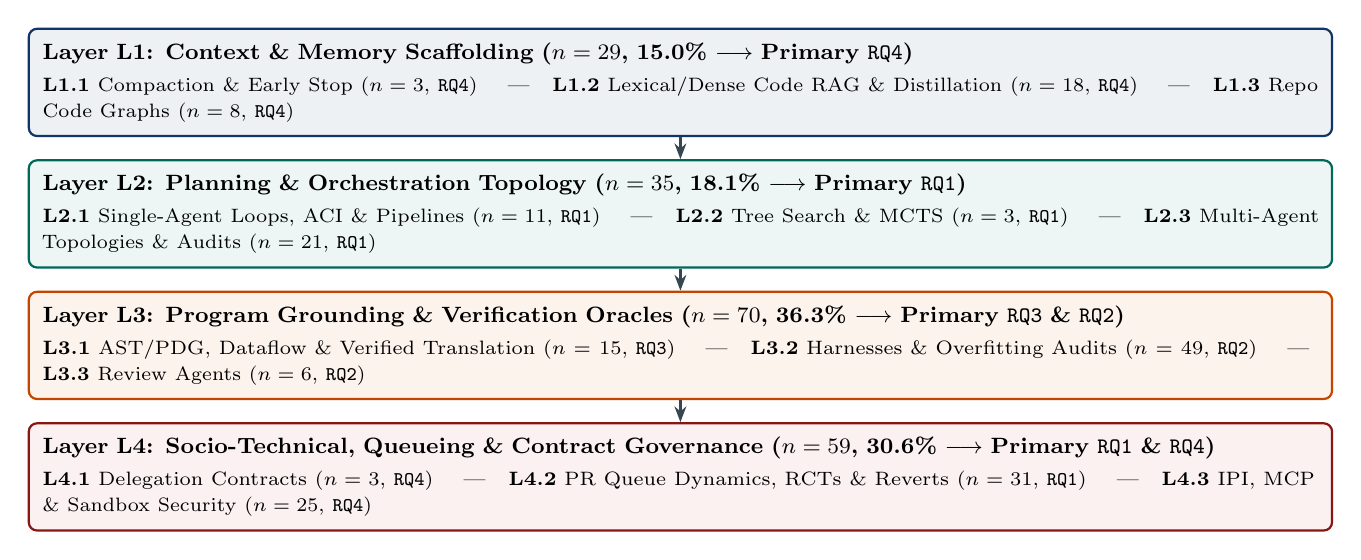
\begin{tikzpicture}[
    node distance=0.28cm,
    layer/.style={rectangle, rounded corners=3pt, draw=navyblue, thick, fill=softgray, text width=16.2cm, minimum height=0.98cm, align=left, font=\footnotesize, inner sep=5pt},
    larr/.style={-{Stealth[length=2.0mm]}, thick, draw=slate}
]
\node[layer, fill=navyblue!7, draw=navyblue] (l1) {
\textbf{Layer L1: Context \& Memory Scaffolding ($n = 29$, 15.0\% $\longrightarrow$ Primary \texttt{RQ4})}\\[2pt]
\scriptsize \textbf{L1.1} Compaction \& Early Stop ($n=3$, \texttt{RQ4}) \quad|\quad \textbf{L1.2} Lexical/Dense Code RAG \& Distillation ($n=18$, \texttt{RQ4}) \quad|\quad \textbf{L1.3} Repo Code Graphs ($n=8$, \texttt{RQ4})};

\node[layer, fill=tealaccent!7, draw=tealaccent!85!black, below=of l1] (l2) {
\textbf{Layer L2: Planning \& Orchestration Topology ($n = 35$, 18.1\% $\longrightarrow$ Primary \texttt{RQ1})}\\[2pt]
\scriptsize \textbf{L2.1} Single-Agent Loops, ACI \& Pipelines ($n=11$, \texttt{RQ1}) \quad|\quad \textbf{L2.2} Tree Search \& MCTS ($n=3$, \texttt{RQ1}) \quad|\quad \textbf{L2.3} Multi-Agent Topologies \& Audits ($n=21$, \texttt{RQ1})};

\node[layer, fill=amber!7, draw=amber!85!black, below=of l2] (l3) {
\textbf{Layer L3: Program Grounding \& Verification Oracles ($n = 70$, 36.3\% $\longrightarrow$ Primary \texttt{RQ3} \& \texttt{RQ2})}\\[2pt]
\scriptsize \textbf{L3.1} AST/PDG, Dataflow \& Verified Translation ($n=15$, \texttt{RQ3}) \quad|\quad \textbf{L3.2} Harnesses \& Overfitting Audits ($n=49$, \texttt{RQ2}) \quad|\quad \textbf{L3.3} Review Agents ($n=6$, \texttt{RQ2})};

\node[layer, fill=crimson!6, draw=crimson!75!black, below=of l3] (l4) {
\textbf{Layer L4: Socio-Technical, Queueing \& Contract Governance ($n = 59$, 30.6\% $\longrightarrow$ Primary \texttt{RQ1} \& \texttt{RQ4})}\\[2pt]
\scriptsize \textbf{L4.1} Delegation Contracts ($n=3$, \texttt{RQ4}) \quad|\quad \textbf{L4.2} PR Queue Dynamics, RCTs \& Reverts ($n=31$, \texttt{RQ1}) \quad|\quad \textbf{L4.3} IPI, MCP \& Sandbox Security ($n=25$, \texttt{RQ4})};

\draw[larr] (l1.south) -- (l2.north);
\draw[larr] (l2.south) -- (l3.north);
\draw[larr] (l3.south) -- (l4.north);
\end{tikzpicture}
\caption{Four-Layer Architectural \& Socio-Technical Taxonomy Ordered Top-to-Bottom (\texttt{L1 $\to$ L4}) Showing Deterministic Sub-Layer-to-Primary-\texttt{RQ} Mapping Across All 193 Studies ($29 + 35 + 70 + 59 = 193$).}
\label{fig:taxonomy}
\end{figure*}

Figure~\ref{fig:taxonomy} orders the 193 primary studies top-to-bottom (\texttt{L1 $\to$ L4}) into a mutually exclusive \textbf{Four-Layer, Twelve-Sub-Layer Taxonomy}, while Table~\ref{tab:rep40} profiles a stratified 40-study subset (20 in \texttt{L1}--\texttt{L2}, 20 in \texttt{L3}--\texttt{L4}):
\begin{itemize}[leftmargin=*,nosep]
    \item \textbf{Layer L1 --- Context \& Memory Scaffolding ($n = 29$, 15.0\%):} \emph{L1.1 Context Window Compaction \& Early Termination} ($n=3$)~\cite{liu2024lost,packer2023memgpt,guo2026eet}; \emph{L1.2 Lexical/Dense Code RAG \& Context Distillation} ($n=18$)~\cite{zhang2023repocoder,zhang2024codeagent,wang2025coderagbench,liu2024marscode,suresh2025cornstack,xie2025swefixer,guo2025repoaudit,yildiz2025benchmarking,ma2025thinking,mu2025experepair,ma2025swegpt,li2026contextbench,zhu2026swe,liu2026racebench,jia2026compressing,zhang2026sweexplore,desai2026swemarathon,lin2026run}; and \emph{L1.3 Structural Repository Graphs \& Paging} ($n=8$)~\cite{zhang2024autocoderover,liu2025codexgraph,ouyang2025repograph,tao2025code,chen2025locagent,chai2026reponav,pu2026typescript,chen2026measure}.
    \item \textbf{Layer L2 --- Planning \& Orchestration Topology ($n = 35$, 18.1\%):} \emph{L2.1 Single-Agent Closed Loops \& ACIs} ($n=11$)~\cite{yao2023react,zhang2023selfedit,schick2023toolformer,shinn2023reflexion,madaan2023selfrefine,chen2024teaching,yang2024sweagent,bouzenia2024repairagent,xia2024demystifying,wang2025openhands,pan2025training}; \emph{L2.2 Deliberate Tree Search \& MCTS} ($n=3$)~\cite{yao2023tree,zhou2024language,antoniades2024swesearch}; and \emph{L2.3 Multi-Agent Collaborative Topologies \& Failure Taxonomies} ($n=21$)~\cite{qian2024chatdev,hong2024metagpt,wu2024autogen,yang2023whitefox,islam2024mapcoder,tao2024magis,huang2024unidebugger,xu2025hallucination,ye2025prompt,cemri2025multiagent,ye2025adverintentagent,oueslati2025refagent,ananiadou2026hiras,zhang2026sgagent,wu2026guessing,ibrahimzada2026recodeagent,zhang2026understanding,peng2026playcoder,tian2026mumutestup,chen2026tracedev,wang2026paichecker}.
    \item \textbf{Layer L3 --- Program Grounding \& Verification Oracles ($n = 70$, 36.3\%):} \emph{L3.1 Static/Neuro-Symbolic AST, Dataflow \& Verified Translation} ($n=15$)~\cite{bairi2024codeplan,yuan2024transagent,wang2024llmdfa,pan2024lost,yang2024vert,yu2024fight,shetty2025syzygy,wang2025cvebench,zan2025multiswebench,li2025patchpilot,fu2025security,garg2026debug2fix,tufano2026developers,ma2026llm,kanvar2026meets}; \emph{L3.2 Execution Harnesses, Mutation Benchmarks \& Overfitting Audits} ($n=49$)~\cite{dong2023selfcollaboration,lemieux2023codamosa,liu2023your,jimenez2024swebench,ma2024alibaba,mndlersasahara2024swtbench,gu2024cruxeval,alshahwan2024automated,jain2025livecodebench,lin2024soen101,trivedi2024appworld,yang2024swebench,aleithan2026swebench,hu2025repo2run,guo2025swe,yang2025swesmith,yu2025utboost,rondon2025evaluating,wang2025solved,jain2025r2egym,rashid2025swepolybench,ceka2025understanding,bouzenia2025understanding,team2025trae,peng2025sweqa,zhong2025impossiblebench,horikawa2025agentic,jin2026chainswe,li2026laboratory,agarwal2026ides,gao2026autopilot,ghaleb2026fingerprinting,cynthia2026all,ottenhof2026agents,martnez2026whats,zhou2026featurebench,gloaguen2026evaluating,khan2026adoption,kong2026compiling,badertdinov2026swerebench,chen2026beyondswe,li2026probe,pham2026synthetic,oukhay2026code,xiang2026empowering,lam2026swechain,hasan2026what,wu2026swetogether,galster2026configuring}; and \emph{L3.3 Automated Code Review Agents} ($n=6$)~\cite{ullah2024llms,tang2024codeagent,popescu2026investigating,charoenwet2026agentic,liu2026e4rreviewer,zheng2026static}.
    \item \textbf{Layer L4 --- Socio-Technical, Queueing \& Contract Governance ($n = 59$, 30.6\%):} \emph{L4.1 Requirements \& Delegated-Autonomy Contracts} ($n=3$)~\cite{arora2026specifying,ciancarini2026charge,feng2026sage}; \emph{L4.2 Developer Productivity RCTs, PR Queue Dynamics \& Merge Friction} ($n=31$)~\cite{asare2023usercentered,becker2025measuring,li2025rise,watanabe2025use,gong2026analyzing,ehsani2026where,ogenrwot2026coding,cynthia2026bug,milanese2026humanagent,huang2026more,alam2026agentinvolved,chen2026commit,li2026aidev,pinna2026comparing,nachuma2026teammates,cui2026effects,ogenrwot2026agenticflict,chowdhury2026industry,khemissi2026humans,hoseinpour2026empirical,haque2026empirical,khelifi2026behind,wang2026aigenerated,watanabe2026coding,fatima2026footprints,gonzalez2026bots,peralta2026agentic,ogenrwot2026patchtrack,chung2026collaborator,gao2026evaluating,adams2026automating}; and \emph{L4.3 Indirect Prompt Injection, MCP \& Runtime Security} ($n=25$)~\cite{pearce2023examining,andriushchenko2024agentdojo,zhan2024injecagent,kapoor2024agents,jia2024task,wang2025agentvigil,zhan2025adaptive,an2025ipiguard,zhu2025melon,zhong2025rtbas,miserendino2025swelancer,shi2025promptarmor,wang2025agentarmor,wen2025hammer,zhang2025mcp,wei2025toward,chang2026overcoming,ghammam2026builds,wang2026landscape,schmotz2026skillinject,he2026attriguard,dziemian2026vulnerable,zhao2026clawguard,weng2026argus,qu2026overeager}.
\end{itemize}

\textbf{Orthogonal Relationship Between Architectural Layers (\texttt{L1}--\texttt{L4}) and Research Questions (\texttt{RQ1}--\texttt{RQ4}).} Fulfilling PRISMA 2020 Item 17, Layers \texttt{L1}--\texttt{L4} classify \emph{where} each technical or socio-technical mechanism sits in the agentic SE stack, whereas Research Questions \texttt{RQ1}--\texttt{RQ4} in Section~\ref{sec:synthesis} examine \emph{cross-layer empirical relationships}. Mapping layers one-to-one onto RQs would obscure key interactions across the stack: analyzing the Productivity--Verification Paradox (\texttt{RQ1}) requires connecting upstream orchestration designs in \texttt{L2} ($n=35$) with downstream PR review-queue telemetry in \texttt{L4.2} ($n=31$, totaling $66$ primary \texttt{RQ1} studies). Likewise, \texttt{L3} separates empirical testing and code-review studies (\texttt{L3.2}--\texttt{L3.3} $\to$ \texttt{RQ2}, $n=55$) from formal program-analysis constraints (\texttt{L3.1} $\to$ \texttt{RQ3}, $n=15$), while production cost and security governance (\texttt{RQ4}, $n=57$) links context management (\texttt{L1}, $n=29$) with delegation contracts and MCP sandboxing (\texttt{L4.1, L4.3}, $n=28$). Because 161 of 193 studies (83.4\%) report metrics spanning multiple RQs, combining a mutually exclusive 12-sub-layer primary assignment (Figure~\ref{fig:taxonomy}, Table~\ref{tab:rqs}) with secondary \texttt{rqs} tags keeps counts exact without losing cross-layer evidence.

\begin{table*}[t!]
\centering
\caption{Stratified Representative Subset ($n = 40$ of $N = 193$, Part I: Layers \texttt{L1}--\texttt{L2}, 20 Studies) Across All Twelve Taxonomy Sub-Layers. The \texttt{RQs} column lists all assigned research-question tags in numerical order (\texttt{RQ1}--\texttt{RQ4}); each study's unique mutually exclusive primary assignment (\texttt{primary\_rq}) and persistent DOI/URL are archived in \texttt{03\_\allowbreak extraction/\allowbreak review\_\allowbreak matrix.\allowbreak csv}.}
\label{tab:rep40}
\scriptsize
\setlength{\tabcolsep}{3.2pt}
\renewcommand{\arraystretch}{0.95}
\begin{tabularx}{\textwidth}{l >{\raggedright\arraybackslash}p{2.65cm} >{\raggedright\arraybackslash}p{2.05cm} c >{\raggedright\arraybackslash}p{1.40cm} X}
\toprule
\textbf{ID} & \textbf{Study} & \textbf{Venue} & \textbf{Sub} & \textbf{RQs} & \textbf{Verified Empirical Scope \& Key Finding} \\
\midrule
S013 & Liu et al. (2024)~\cite{liu2024lost} & TACL & L1.1 & RQ4 & Multi-doc \& KV long-context probe; severe mid-context recall drop (U-shaped curve). \\
S021 & Packer et al. (2023)~\cite{packer2023memgpt} & arXiv & L1.1 & RQ4 & OS-inspired virtual context paging between fast prompt memory and external storage. \\
S106 & Guo et al. (2026)~\cite{guo2026eet} & Findings of ACL & L1.1 & RQ4 & Experience-driven early termination; cuts SE agent total cost by 19\%-55\% (32\% avg, <=0.2\% loss). \\
S005 & Zhang et al. (2023)~\cite{zhang2023repocoder} & EMNLP & L1.2 & RQ3, RQ4 & Iterative retrieval-generation loop for repository-level code completion. \\
S045 & Wang et al. (2025)~\cite{wang2025coderagbench} & Findings of NAACL & L1.2 & RQ3, RQ4 & CodeRAG-Bench across competition, open-domain, and repository retrieval settings. \\
S146 & Jia et al. (2026)~\cite{jia2026compressing} & ASE & L1.2 & RQ1, RQ4 & Oracle-guided context distillation (SWEzze); \textasciitilde{}6x compression, -51.8\% to -71.3\% token budget. \\
S040 & Zhang et al. (2024)~\cite{zhang2024autocoderover} & ISSTA & L1.3 & RQ1, RQ3, RQ4 & AST-aware iterative search + SBFL; resolves 19\% of SWE-bench Lite at \$0.43 avg cost. \\
S050 & Liu et al. (2025)~\cite{liu2025codexgraph} & NAACL & L1.3 & RQ1, RQ3, RQ4 & Code graph database interface bridging LLM agents with multi-file repository symbol graphs. \\
S052 & Ouyang et al. (2025)~\cite{ouyang2025repograph} & ICLR & L1.3 & RQ1, RQ3, RQ4 & Repository-level line/symbol dependency graph plug-in boosting SWE-bench agents. \\
S079 & Chen et al. (2025)~\cite{chen2025locagent} & ACL & L1.3 & RQ1, RQ3, RQ4 & Heterogeneous code graphs; 92.7\% file localization at \textasciitilde{}86\% lower localization cost (+12\% Pass@10). \\
S001 & Yao et al. (2023)~\cite{yao2023react} & ICLR & L2.1 & RQ1, RQ3 & Interleaved reasoning traces and environment action execution in closed-loop agents. \\
S004 & Shinn et al. (2023)~\cite{shinn2023reflexion} & NeurIPS & L2.1 & RQ1, RQ3 & Verbal reinforcement memory over execution feedback without weight updates. \\
S029 & Yang et al. (2024)~\cite{yang2024sweagent} & NeurIPS & L2.1 & RQ1, RQ3 & Agent-Computer Interface (ACI) design; 12.5\% Pass@1 on SWE-bench and 87.7\% on HumanEvalFix. \\
S047 & Xia et al. (2024)~\cite{xia2024demystifying} & PACMSE (FSE) & L2.1 & RQ1, RQ2, RQ3, RQ4 & Three-stage Agentless pipeline; 32.00\% (96 fixes) on SWE-bench Lite at \$0.70/issue. \\
S012 & Yao et al. (2023)~\cite{yao2023tree} & NeurIPS & L2.2 & RQ1, RQ3, RQ4 & Deliberate lookahead tree search with self-evaluated intermediate thought states. \\
S019 & Zhou et al. (2024)~\cite{zhou2024language} & ICML & L2.2 & RQ1, RQ3 & Monte Carlo tree search unifying reasoning, acting, and reflection (LATS). \\
S055 & Antoniades et al. (2024)~\cite{antoniades2024swesearch} & arXiv & L2.2 & RQ1, RQ3 & MCTS + iterative value-function refinement for repository issue resolution. \\
S015 & Hong et al. (2024)~\cite{hong2024metagpt} & ICLR & L2.3 & RQ1, RQ4 & SOP-structured multi-agent software roles reducing cascading chat hallucinations. \\
S014 & Qian et al. (2024)~\cite{qian2024chatdev} & ACL & L2.3 & RQ1, RQ4 & Waterfall role-play communicative agents with dehallucination dialogues. \\
S081 & Cemri et al. (2025)~\cite{cemri2025multiagent} & NeurIPS & L2.3 & RQ1, RQ4 & MAST audit of 1,600+ traces across 7 MAS frameworks (kappa=0.88; 14 failure modes). \\
\bottomrule
\end{tabularx}
\end{table*}
\addtocounter{table}{-1}
\begin{table*}[t!]
\centering
\caption{Continued --- Stratified Representative Subset ($n = 40$ of $N = 193$, Part II: Layers \texttt{L3}--\texttt{L4}, 20 Studies).}
\scriptsize
\setlength{\tabcolsep}{3.2pt}
\renewcommand{\arraystretch}{0.95}
\begin{tabularx}{\textwidth}{l >{\raggedright\arraybackslash}p{2.65cm} >{\raggedright\arraybackslash}p{2.05cm} c >{\raggedright\arraybackslash}p{1.40cm} X}
\toprule
\textbf{ID} & \textbf{Study} & \textbf{Venue} & \textbf{Sub} & \textbf{RQs} & \textbf{Verified Empirical Scope \& Key Finding} \\
\midrule
S035 & Wang et al. (2024)~\cite{wang2024llmdfa} & NeurIPS & L3.1 & RQ3 & Compilation-free neuro-symbolic dataflow analysis; 87.10\% precision, 80.77\% recall. \\
S043 & Yang et al. (2024)~\cite{yang2024vert} & ASE & L3.1 & RQ3 & Wasm-oracle + BMS Rust transpilation (1,394 programs); model-checking 1\% -> 42\%. \\
S041 & Pan et al. (2024)~\cite{pan2024lost} & ICSE & L3.1 & RQ2, RQ3 & 1,700 cross-PL translations; 2.1\%-47.3\% accuracy across 15 bug categories (+5.5\% repair). \\
S074 & Li et al. (2025)~\cite{li2025patchpilot} & ICML & L3.1 & RQ1, RQ3, RQ4 & Rule-guided 5-stage SE agent with formal/refinement validation under \$1/issue. \\
S020 & Jimenez et al. (2024)~\cite{jimenez2024swebench} & ICLR & L3.2 & RQ1, RQ2, RQ3 & 2,294 real GitHub issues across 12 Python repos; non-agentic baseline solves 1.96\%. \\
S054 & Aleithan et al. (2026)~\cite{aleithan2026swebench} & ACM AIware & L3.2 & RQ1, RQ2, RQ3 & Uncovers 32.67\% solution leakage \& 31.08\% weak tests; filtered rate 12.47\% -> 3.97\%. \\
S070 & Yu et al. (2025)~\cite{yu2025utboost} & ACL & L3.2 & RQ1, RQ2, RQ3 & Finds 345 erroneous passed SWE-bench patches; alters 40.9\% Lite \& 24.4\% Verified ranks. \\
S082 & Wang et al. (2025)~\cite{wang2025solved} & ICSE & L3.2 & RQ1, RQ2, RQ3 & PatchDiff reveals 29.6\% behavioral divergence \& +6.4 pp SWE-bench Verified inflation. \\
S030 & M{\"u}ndler-Sasahara et al. (2024)~\cite{mndlersasahara2024swtbench} & NeurIPS & L3.2 & RQ2, RQ3 & SWT-Bench issue-to-test synthesis; generated reproducing tests double SWE-agent precision. \\
S023 & Ullah et al. (2024)~\cite{ullah2024llms} & IEEE S\&P & L3.3 & RQ2, RQ4 & SecLLMHolmes (228 scenarios); identifier renaming flips 17\%-26\% of security verdicts. \\
S189 & Zheng et al. (2026)~\cite{zheng2026static} & PACMSE (FSE) & L3.3 & RQ2, RQ4 & MCR-Bench (2,269 multi-round review tasks across 5 languages); sharp multi-round decay. \\
S187 & Liu et al. (2026)~\cite{liu2026e4rreviewer} & PACMSE (FSE) & L3.3 & RQ2, RQ3 & End-to-end GRPO reasoning-aligned review; 74.61\% quality F1 and +22.96\% CodeBLEU. \\
S184 & Arora et al. (2026)~\cite{arora2026specifying} & ASE & L4.1 & RQ3, RQ4 & Agency Justification Record \& graduated Agentic Delegation Policy for RE boundaries. \\
S193 & Feng et al. (2026)~\cite{feng2026sage} & MAS-GAIN (ASE) & L4.1 & RQ3, RQ4 & 3 co-evolving sources \& 10 declarative transition guards for requirements sign-off. \\
S140 & Cui et al. (2026)~\cite{cui2026effects} & Management Science & L4.2 & RQ1, RQ2 & 3-firm RCT (N = 4,867 developers); +26.08\% completed tasks (SE 10.3\%). \\
S190 & Adams et al. (2026)~\cite{adams2026automating} & ASE & L4.2 & RQ1, RQ2, RQ4 & Meta RADAR (535K+ reviewed, 331K+ landed); +105.9\% LoC/diff YoY, >4.3x faster close. \\
S110 & Gong et al. (2026)~\cite{gong2026analyzing} & MSR & L4.2 & RQ1, RQ2 & 23,247 agentic PRs; high message-code mismatch inflates merge time 3.5x (55.8 vs 16.0 hrs). \\
S096 & Watanabe et al. (2025)~\cite{watanabe2025use} & ACM TOSEM & L4.2 & RQ1, RQ2 & 567 Claude Code PRs across 157 OSS repos; 83.8\% merged, 45.1\% require human edits. \\
S027 & Zhan et al. (2024)~\cite{zhan2024injecagent} & Findings of ACL & L4.3 & RQ4 & 1,054 indirect prompt injection cases across 30 agents; 24\% GPT-4 base ASR. \\
S100 & Zhang et al. (2025)~\cite{zhang2025mcp} & arXiv & L4.3 & RQ4 & MCP Security Bench (405 tools, 2,000 attacks); stronger models show higher susceptibility. \\
\bottomrule
\end{tabularx}
\end{table*}
\begin{table*}[t!]
\centering
\caption{Provenance, Publication Venue, Study Design, Sample Scope, and Abstract-Verified Metrics of Headline Quantitative Claims (extracted from \texttt{03\_\allowbreak extraction/\allowbreak verified\_\allowbreak evidence\_\allowbreak ledger.\allowbreak csv}).}
\label{tab:provenance}
\scriptsize
\setlength{\tabcolsep}{3.5pt}
\begin{tabularx}{\textwidth}{>{\raggedright\arraybackslash}p{2.45cm} >{\raggedright\arraybackslash}p{1.85cm} >{\raggedright\arraybackslash}p{2.30cm} >{\raggedright\arraybackslash}p{2.80cm} X}
\toprule
\textbf{Study} & \textbf{Venue} & \textbf{Design} & \textbf{Sample / Cohort} & \textbf{Abstract-Verified Empirical Metric} \\
\midrule
Cui et al. (2026)~\cite{cui2026effects} & Management Science & Multi-enterprise RCT & N = 4,867 developers across 3 firms & +26.08\% completed tasks (SE 10.3\%) across 3 experiments and 4,867 developers \\
Becker et al. (2025)~\cite{becker2025measuring} & arXiv & Open-source developer RCT & 16 experienced OSS developers, 246 tasks (\textasciitilde{}5 yrs project experience) & 16 developers complete 246 tasks (avg 5 years prior experience) \\
Adams et al. (2026)~\cite{adams2026automating} & ASE & Industrial telemetry \& DiD & 535K+ RADAR-reviewed diffs at Meta (331K+ landed) & +105.9\% YoY LoC/diff; +51\% diff volume (>80\% agentic); 535K+ reviewed \& 331K+ landed; >4.3x faster close, -35\% review wall time \\
Gong et al. (2026)~\cite{gong2026analyzing} & MSR & Empirical GitHub PR review study & 23,247 agentic PRs across 5 agents (974 manually annotated) & 1.7\% high message-code inconsistency (406 PRs; 45.4\% unimplemented claims) -> 51.7\% lower acceptance (28.3\% vs. 80.0\%) \& 3.5x merge time (55.8 vs. 16.0 hours) \\
Watanabe et al. (2025)~\cite{watanabe2025use} & ACM TOSEM & Empirical GitHub PR study & 567 Claude Code PRs across 157 OSS projects & 567 PRs across 157 projects: 83.8\% merged; 54.9\% unmodified, 45.1\% of merged PRs require human revisions \\
Oukhay et al. (2026)~\cite{oukhay2026code} & MSR & Empirical post-merge revert study & 33,580 agentic PRs (86,315 commits) across 5 agents & 2.66\% PR revert rate across 33,580 PRs (0.7\% Codex to 7.6\% Copilot); 22.33\% side effects, 22.13\% overengineering, 17.71\% incorrectness, 12.47\% dependencies \\
Chowdhury et al. (2026)~\cite{chowdhury2026industry} & MSR & Empirical PR review study & 3,109 commented PRs from AIDev (98 closed CRA-only) & CRA-only merge rate 45.20\% vs. 68.37\% human-only (-23.17 pp); 12 of 13 CRAs <60\% signal ratio \\
Aleithan et al. (2026)~\cite{aleithan2026swebench} & ACM AIware & Benchmark contamination \& oracle audit & SWE-bench audit of SWE-Agent+GPT-4 patches & 32.67\% solution leakage, 31.08\% weak tests, >94\% pre-cutoff; filtered resolve rate drops 12.47\% -> 3.97\% \\
Yu et al. (2025)~\cite{yu2025utboost} & ACL & Automated test-oracle augmentation & SWE-Bench Lite \& Verified leaderboard audit & 36 insufficient-test tasks \& 345 erroneous passed patches; impacts 40.9\% Lite \& 24.4\% Verified entries (18 \& 11 rank changes) \\
Wang et al. (2025)~\cite{wang2025solved} & ICSE & Differential patch testing (PatchDiff) & SWE-bench Verified plausible patches across 3 tools & 7.8\% fail developer tests; 29.6\% behaviorally divergent; 28.6\% of divergent certainly incorrect; +6.4 pp resolution inflation \\
Rondon et al. (2025)~\cite{rondon2025evaluating} & ICSE & Enterprise agentic APR study & 178 Google bugs (78 human-, 100 machine-reported) & 178 bugs (78 human, 100 machine): plausible 73\% / 25.6\% vs. semantically equivalent 43\% / 17.9\% \\
Yang et al. (2024)~\cite{yang2024vert} & ASE & Model-checked Rust transpilation & 1,394 programs transpiled to Rust & 1,394 programs: property-based testing 31\% -> 54\%; bounded model-checking 1\% -> 42\% \\
Chen et al. (2025)~\cite{chen2025locagent} & ACL & Graph-guided localization benchmark & Heterogeneous code graphs with Qwen-2.5-Coder-32B & \textasciitilde{}86\% localization cost reduction, 92.7\% file-level accuracy, +12\% Pass@10 issue resolution \\
Jia et al. (2026)~\cite{jia2026compressing} & ASE & Oracle-guided context compression & SWE-bench Verified across 3 frontier LLMs & \textasciitilde{}6x compression, -51.8\% to -71.3\% total token budget, +5.0\% to +9.2\% resolution rate \\
\bottomrule
\end{tabularx}
\end{table*}

\section{Empirical Synthesis Across Research Questions}
\label{sec:synthesis}

\subsection{RQ1: Delivery Paradox, PR Merge Dynamics, and Orchestration Topologies}
\label{sec:rq1}

% --- FIGURE 3: DELIVERY PARADOX & QUEUE SATURATION (DIVERGING BAR + EXPLICIT LEGEND) ---
\begin{figure*}[t!]
\centering
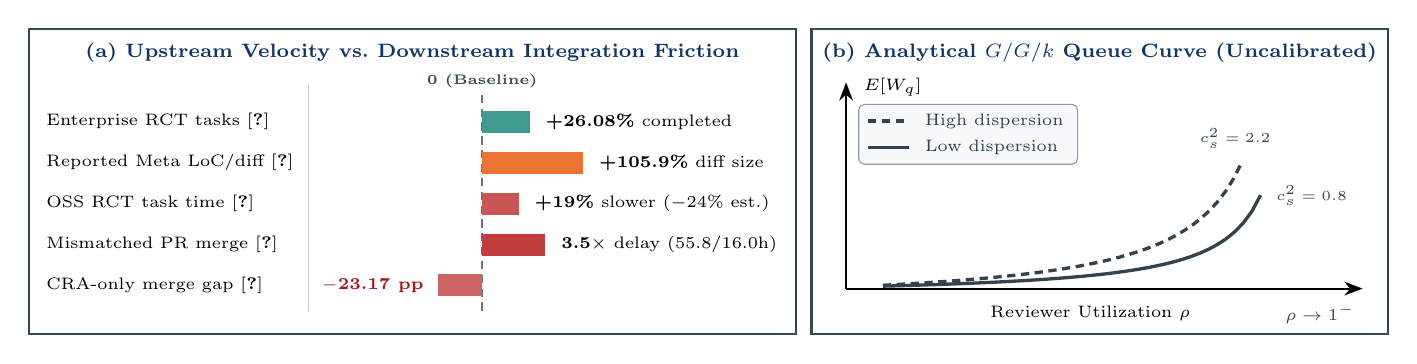
\begin{tikzpicture}[font=\fontsize{6.5}{8.0}\selectfont]
% Left panel: Diverging Horizontal Bar Chart (Zero Baseline at x = 5.76)
\draw[thick, draw=slate] (0,0) rectangle (9.74,3.88);
\node[font=\scriptsize\bfseries, text=navyblue] at (4.87,3.58) {(a) Upstream Velocity vs.\ Downstream Integration Friction};
\draw[slate!30] (3.55,0.30) -- (3.55,3.16);
\draw[slate!75, densely dashed, thick] (5.76,0.30) -- (5.76,3.08);
\node[font=\tiny\bfseries, text=slate] at (5.76,3.22) {0 (Baseline)};

\node[anchor=west] at (0.10,2.70) {Enterprise RCT tasks~\cite{cui2026effects}};
\fill[tealaccent!75] (5.76,2.56) rectangle (6.36,2.84);
\node[anchor=west] at (6.44,2.70) {\textbf{+26.08\%} completed};

\node[anchor=west] at (0.10,2.18) {Reported Meta LoC/diff~\cite{adams2026automating}};
\fill[amber!80] (5.76,2.04) rectangle (7.04,2.32);
\node[anchor=west] at (7.12,2.18) {\textbf{+105.9\%} diff size};

\node[anchor=west] at (0.10,1.66) {OSS RCT task time~\cite{becker2025measuring}};
\fill[crimson!75] (5.76,1.52) rectangle (6.22,1.80);
\node[anchor=west] at (6.30,1.66) {\textbf{+19\%} slower ($-24\%$ est.)};

\node[anchor=west] at (0.10,1.14) {Mismatched PR merge~\cite{gong2026analyzing}};
\fill[crimson!85] (5.76,1.00) rectangle (6.56,1.28);
\node[anchor=west] at (6.64,1.14) {\textbf{3.5$\times$} delay (55.8/16.0h)};

\node[anchor=west] at (0.10,0.62) {CRA-only merge gap~\cite{chowdhury2026industry}};
\fill[crimson!68] (5.20,0.48) rectangle (5.76,0.76);
\node[anchor=east, text=crimson!90!black] at (5.14,0.62) {\textbf{$-$23.17 pp}};

% Right panel: Analytical Uncalibrated G/G/k Queueing Curve with Compact Monochrome Line Legend
\draw[thick, draw=slate] (9.94,0) rectangle (17.26,3.88);
\node[font=\scriptsize\bfseries, text=navyblue] at (13.60,3.58) {(b) Analytical $G/G/k$ Queue Curve (Uncalibrated)};
\draw[-{Stealth}, thick] (10.38,0.58) -- (16.94,0.58);
\draw[-{Stealth}, thick] (10.38,0.58) -- (10.38,3.20);
\node[anchor=west] at (10.48,3.14) {$E[W_q]$};

\draw[very thick, slate!95!black, domain=0.08:0.90, samples=45] plot ({10.38 + 5.85*\x}, {0.60 + 0.13*(\x/(1-\x))});
\draw[very thick, slate!95!black, densely dashed, domain=0.08:0.86, samples=45] plot ({10.38 + 5.85*\x}, {0.60 + 0.26*(\x/(1-\x))});

% Compact Legend ordered top-to-bottom matching curve height (well clear of curves, monochrome line-style distinction)
\filldraw[fill=softgray!85, draw=slate!55, rounded corners=2pt] (10.54,2.16) rectangle (13.32,2.92);
\draw[very thick, slate!95!black, densely dashed] (10.66,2.71) -- (11.18,2.71);
\node[text=slate!95!black, anchor=west] at (11.26,2.71) {High dispersion};
\draw[very thick, slate!95!black] (10.66,2.37) -- (11.18,2.37);
\node[text=slate!95!black, anchor=west] at (11.26,2.37) {Low dispersion};

\node[font=\tiny\bfseries, text=slate!95!black, anchor=south] at (15.32,2.24) {$c_s^2 = 2.2$};
\node[font=\tiny\bfseries, text=slate!95!black, anchor=west] at (15.72,1.76) {$c_s^2 = 0.8$};

\node[anchor=center] at (13.48,0.26) {Reviewer Utilization $\rho$};
\node[slate, anchor=center] at (16.40,0.26) {$\rho \to 1^-$};
\end{tikzpicture}
\caption{Empirical and Analytical Queueing Anatomy of the Productivity--Verification Paradox (Panel~(a) plots reported effect sizes around a zero baseline, with negative changes extending leftward; Panel~(b) plots illustrative Kingman-regime curves from Eq.~\eqref{eq:kingman} for high review-service dispersion $c_s^2=2.2$ [dashed] vs.\ low dispersion $c_s^2=0.8$ [solid]).}
\label{fig:paradox}
\end{figure*}
\begin{table*}[t!]
\centering
\caption{Synthesis of Agentic Orchestration Topologies and Real-World Pull-Request Integration Outcomes (RQ1).}
\label{tab:rq1_topologies}
\scriptsize
\setlength{\tabcolsep}{3.8pt}
\begin{tabularx}{\textwidth}{>{\raggedright\arraybackslash}p{2.20cm} >{\raggedright\arraybackslash}p{2.85cm} >{\raggedright\arraybackslash}p{2.30cm} X}
\toprule
\textbf{Paradigm / Cohort} & \textbf{Representative Studies} & \textbf{Benchmark / Scale} & \textbf{Verified Performance, Cost \& Bottleneck Profile} \\
\midrule
Single-Agent ACI Loop & SWE-agent~\cite{yang2024sweagent}, OpenHands~\cite{wang2025openhands} & SWE-bench / 15 benchmarks & Custom ACI achieves 12.5\% Pass@1 on SWE-bench and 87.7\% on HumanEvalFix; OpenHands evaluates 15 tasks. \\
Fixed 3-Stage Pipeline & Agentless~\cite{xia2024demystifying}, PatchPilot~\cite{li2025patchpilot} & SWE-bench Lite / Verified & Agentless hits 32.00\% (96 fixes) at \$0.70/issue; PatchPilot adds rule-based refinement under \$1/issue. \\
Tree Search / MCTS & ToT~\cite{yao2023tree}, LATS~\cite{zhou2024language}, SWE-Search~\cite{antoniades2024swesearch} & HumanEval / SWE-bench & Multi-branch exploration improves hard localization/repair but multiplies token trajectories without pruning. \\
Multi-Agent Role-Play & MetaGPT~\cite{hong2024metagpt}, ChatDev~\cite{qian2024chatdev}, MAST~\cite{cemri2025multiagent} & 1,600+ MAS traces ($\kappa=0.88$) & SOPs curb chat drift, yet MAST uncovers 14 failure modes across design, misalignment, and verification. \\
Sequential \& Feature SE & ChainSWE~\cite{jin2026chainswe}, FeatureBench~\cite{zhou2026featurebench} & 304 chains / 200 features & Up to 70\% decay across dependent bug chains; 74.4\% SWE-bench model drops to 11.0\% on multi-PR features. \\
OSS \& Industrial PRs & Watanabe~\cite{watanabe2025use}, Gong~\cite{gong2026analyzing}, RADAR~\cite{adams2026automating} & $n=567$ to 535K+ reviewed & 83.8\% Claude PR merge ($n=567$, 45.1\% human-edited); 3.5$\times$ merge delay on mismatched PRs; RADAR 331K+ landed. \\
\bottomrule
\end{tabularx}
\end{table*}

\textbf{1) Task-Level Acceleration vs.\ Repository-Level Slowdown.} Results across \textbf{66 primary \texttt{RQ1} studies} and 111 multi-label \texttt{RQ1}-tagged studies (Table~\ref{tab:rqs}) help explain why AI productivity estimates diverge across settings (Figure~\ref{fig:paradox}, Table~\ref{tab:provenance}). In enterprise environments centered on bounded coding tasks and inline autocomplete, Cui et al.~\cite{cui2026effects} pool field RCTs across Microsoft, Accenture, and an anonymous Fortune 100 company ($N=4,867$ developers) and report a \textbf{+26.08\%} increase (SE 10.3\%) in completed tasks, with larger gains among junior developers. By contrast, in a randomized trial of 16 experienced open-source maintainers working on 246 real issues in mature repositories where they averaged five years of prior experience, Becker et al.~\cite{becker2025measuring} find that early-2025 AI tools \emph{increased} completion time by \textbf{+19\%}, reversing both pre-task expectations ($-24\%$) and post-task self-estimates ($-20\%$).

\textbf{2) Queueing Friction, Message--Code Mismatch, and Reverts in Agentic PRs.} Large-scale repository mining from 2025--2026 tracks what happens when higher patch output meets human review queues (Eq.~\eqref{eq:kingman}). Li et al.~\cite{li2026aidev} release \texttt{AIDev}, covering \textbf{932,791} agent-authored PRs across 116,211 GitHub repositories and 72,189 developers from five tools (OpenAI Codex, Devin, GitHub Copilot, Cursor, and Claude Code). Across \textbf{$n=567$} Claude Code PRs in \textbf{157} open-source projects, Watanabe et al.~\cite{watanabe2025use} observe an 83.8\% merge rate, yet \textbf{45.1\%} of merged PRs required human edits for bug fixes, documentation, or style conventions. In an analysis of \textbf{23,247} agentic PRs across five coding agents (including \textbf{974} manually annotated PRs), Gong et al.~\cite{gong2026analyzing} identify high message--code inconsistency in \textbf{406 PRs (1.7\%)}---with ``descriptions claim unimplemented changes'' making up \textbf{45.4\%} across eight categories---and find that inconsistent PRs incur \textbf{3.5$\times$ longer median merge times} (55.8 vs.\ 16.0 hours) and \textbf{51.7\% lower acceptance} (28.3\% vs.\ 80.0\%). Milanese et al.~\cite{milanese2026humanagent} compare \textbf{6,582} human-agent PRs (HAPRs) with \textbf{3,122} human PRs (HPRs) in \texttt{AIDev}: test-inclusion rates are similar (\textbf{42.9\%} vs.\ \textbf{40.0\%}), but HAPRs nearly double the test-to-source line ratio and add new tests more frequently during co-evolution (\textbf{OR = 1.79}), while Huang et al.~\cite{huang2026more} observe that LLM agents frequently disregard code reuse opportunities, introducing higher redundancy and silent technical debt. Post-merge reliability studies in \texttt{L3.2} (primary \texttt{RQ2}, multi-tagged \texttt{RQ1,RQ2}) add further context: Oukhay et al.~\cite{oukhay2026code} examine 33,580 agentic PRs (86,315 commits) and report a \textbf{2.66\%} revert rate (from 0.7\% for Codex to 7.6\% for Copilot), most often due to \emph{unintended side effects} (22.33\%) and \emph{overengineering} (22.13\%). Because observational OSS PR cohorts~\cite{gong2026analyzing,oukhay2026code,watanabe2025use} do not randomize task assignment and Oukhay et al.\ lack a matched human-PR revert baseline, task complexity and contributor familiarity remain important confounders. Complementary studies by Ehsani et al.~\cite{ehsani2026where} (33k agent-authored PRs across five coding agents, with 600 PRs qualitatively analyzed) and Wang and Yang~\cite{wang2026aigenerated} (1,779 rejected PRs---594 AI-generated and 1,185 human-authored---classified into a 10-category taxonomy) likewise report that rejected AI PRs frequently stem from CI/CD validation failures, incomplete implementations, and inadequate testing. Delegating review entirely to uncalibrated bots can also backfire: across 3,109 commented PRs, Chowdhury et al.~\cite{chowdhury2026industry} find a \textbf{45.20\%} merge rate for bot-only reviews versus \textbf{68.37\%} for human-only reviews ($-23.17$ pp), with 12 of 13 review bots scoring below a 60\% signal ratio. By contrast, in an evaluation of Meta's \texttt{RADAR} system across \textbf{535K+ reviewed diffs} (\textbf{331K+ landed}), Adams et al.~\cite{adams2026automating} report that \emph{risk-tiered} gating (combining eligibility filters, an ML Diff Risk Score, LLM review, and static checks) closes low-risk diffs $>4.3\times$ faster at the median, cuts review wall time by 35\%, and lowers revert and production incident rates to 1/3 and 1/50 of non-RADAR diffs.

\textbf{3) Single-Agent ACIs vs.\ Multi-Agent Topologies and Horizon Decay.} On the architectural side (Table~\ref{tab:rq1_topologies}), closed-loop tool use and verbal reflection~\cite{yao2023react,schick2023toolformer,shinn2023reflexion,madaan2023selfrefine,chen2024teaching,zhang2023selfedit} laid the groundwork for dedicated SE agents, including \texttt{SWE-agent} (\textbf{12.5\%} Pass@1 on SWE-bench and \textbf{87.7\%} on HumanEvalFix via a tailored ACI~\cite{yang2024sweagent}), \texttt{RepairAgent} (guiding tool calls and patch validation through a finite-state machine~\cite{bouzenia2024repairagent}), \texttt{OpenHands}~\cite{wang2025openhands}, and RL-trained \texttt{SWE-Gym} (+19\% absolute resolve gain~\cite{pan2025training}). At the same time, Xia et al.~\cite{xia2024demystifying} show with \texttt{Agentless} (primary \texttt{RQ1}, multi-tagged \texttt{RQ1,RQ3}) that a fixed three-stage localization--repair--validation pipeline resolves 32.00\% of SWE-bench Lite at \$0.70/issue, providing a strong low-cost baseline alongside open-ended agent loops. Role-structured multi-agent frameworks (\texttt{MetaGPT}~\cite{hong2024metagpt}, \texttt{ChatDev}~\cite{qian2024chatdev}, \texttt{AutoGen}~\cite{wu2024autogen}) organize task handoffs, yet Cemri et al.~\cite{cemri2025multiagent} examine 1,600+ traces across seven frameworks (\texttt{MAST}, inter-annotator $\kappa = 0.88$) and catalog 14 recurring failure modes across system design, inter-agent coordination, and verification. Performance also drops substantially beyond single-PR bug fixes: on \texttt{FeatureBench} (200 multi-commit features across 3,825 environments), Zhou et al.~\cite{zhou2026featurebench} report that a model scoring \textbf{74.4\%} on SWE-bench resolves \textbf{11.0\%} of end-to-end feature tasks, and Jin et al.~\cite{jin2026chainswe} report on \texttt{ChainSWE} (304 sequential issues across 54 Python projects) up to a \textbf{70\%} drop in resolution rate as issue chains lengthen.

\subsection{RQ2: Verification Gaps in Automated Testing and Code Review}
\label{sec:rq2}

% --- FIGURE 4: VERIFICATION CHASM & ORACLE INFLATION ---
\begin{figure*}[t!]
\centering
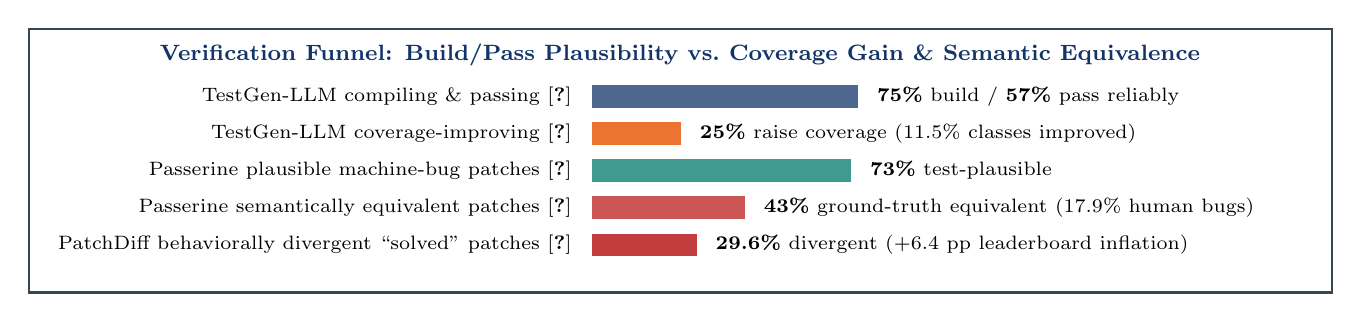
\begin{tikzpicture}[font=\scriptsize]
\draw[thick, draw=slate] (0,0) rectangle (16.55,3.35);
\node[font=\footnotesize\bfseries, text=navyblue] at (8.27,3.02) {Verification Funnel: Build/Pass Plausibility vs.\ Coverage Gain \& Semantic Equivalence};

% Funnel bars (100% = 4.5cm width starting at x = 7.15)
\fill[navyblue!75] (7.15,2.35) rectangle (10.53,2.63);
\node[anchor=east] at (7.02,2.49) {TestGen-LLM compiling \& passing~\cite{alshahwan2024automated}};
\node[anchor=west] at (10.65,2.49) {\textbf{75\%} build / \textbf{57\%} pass reliably};

\fill[amber!80] (7.15,1.88) rectangle (8.28,2.16);
\node[anchor=east] at (7.02,2.02) {TestGen-LLM coverage-improving~\cite{alshahwan2024automated}};
\node[anchor=west] at (8.40,2.02) {\textbf{25\%} raise coverage (11.5\% classes improved)};

\fill[tealaccent!75] (7.15,1.41) rectangle (10.44,1.69);
\node[anchor=east] at (7.02,1.55) {Passerine plausible machine-bug patches~\cite{rondon2025evaluating}};
\node[anchor=west] at (10.56,1.55) {\textbf{73\%} test-plausible};

\fill[crimson!75] (7.15,0.94) rectangle (9.09,1.22);
\node[anchor=east] at (7.02,1.08) {Passerine semantically equivalent patches~\cite{rondon2025evaluating}};
\node[anchor=west] at (9.21,1.08) {\textbf{43\%} ground-truth equivalent (17.9\% human bugs)};

\fill[crimson!85] (7.15,0.47) rectangle (8.48,0.75);
\node[anchor=east] at (7.02,0.61) {PatchDiff behaviorally divergent ``solved'' patches~\cite{wang2025solved}};
\node[anchor=west] at (8.60,0.61) {\textbf{29.6\%} divergent (+6.4 pp leaderboard inflation)};
\end{tikzpicture}
\caption{Empirical Verification Funnel Reported Across Industrial Test Generation and Repository Program Repair Studies.}
\label{fig:verification}
\end{figure*}

\textbf{1) Benchmark Contamination, Weak Tests, and Patch Overfitting.} Evidence across \textbf{55 primary \texttt{RQ2} studies} (94 multi-label \texttt{RQ2}-tagged studies) shows that pass rates on static regression suites often overstate semantic patch correctness (Figure~\ref{fig:verification}). Building on \texttt{SWE-bench}~\cite{jimenez2024swebench}, Aleithan et al.~\cite{aleithan2026swebench} (\texttt{SWE-Bench+}) find that \textbf{32.67\%} of resolved patches draw on solution hints in issue descriptions or comments and \textbf{31.08\%} pass incomplete tests, adjusting \texttt{SWE-Agent+GPT-4} resolution from 12.47\% to \textbf{3.97\%}. Through automated test augmentation in \texttt{UTBoost}, Yu et al.~\cite{yu2025utboost} identify \textbf{345} under-tested patches previously marked as resolved, shifting \textbf{40.9\%} of SWE-Bench Lite and \textbf{24.4\%} of SWE-Bench Verified leaderboard entries (18 and 11 rank changes). Using differential testing (\texttt{PatchDiff}), Wang et al.~\cite{wang2025solved} find that 7.8\% of ``solved'' Verified patches fail developer test suites and \textbf{29.6\%} diverge behaviorally from reference fixes (28.6\% confirmed incorrect), inflating reported solve rates by \textbf{6.4 percentage points}. Industrial repair evaluations report similar gaps: on 178 internal Google bugs, Rondon et al.~\cite{rondon2025evaluating} observe that \texttt{Passerine} generates test-passing patches for \textbf{73\%} of machine-reported and \textbf{25.6\%} of human-reported bugs, whereas manual review confirms semantic equivalence for \textbf{43\%} and \textbf{17.9\%}. Under specification--test conflicts where agents have write permissions on test files (\texttt{ImpossibleBench}), Zhong et al.~\cite{zhong2025impossiblebench} further observe that agents may satisfy checks by modifying or removing failing assertions.

\textbf{2) Build/Pass Plausibility vs.\ Coverage Adequacy in Test Synthesis.} Hybrid search (\texttt{CodaMosa}~\cite{lemieux2023codamosa}), test-input amplification (\texttt{EvalPlus}~\cite{liu2023your}), rolling contamination-resistant benchmarks (\texttt{LiveCodeBench} across 400 contest problems~\cite{jain2025livecodebench}), and issue-to-test generation (\texttt{SWT-Bench}, which doubles \texttt{SWE-agent} precision when used as a patch filter~\cite{mndlersasahara2024swtbench}) show the value of targeted test synthesis. At production scale, Alshahwan et al.~\cite{alshahwan2024automated} report the filtering funnel observed with Meta's \texttt{TestGen-LLM} (Figure~\ref{fig:verification}): \textbf{75\%} of generated test classes build, \textbf{57\%} pass reliably without flakiness, and \textbf{25\%} increase coverage (improving 11.5\% of target classes, with 73\% engineer acceptance after execution filtering). Without mutation or differential checks, passing an existing or generated test suite alone does not guarantee behavioral equivalence.

\textbf{3) Automated Code Review Fragility and Human Trust Calibration.} Code-review studies in \texttt{L3.3} highlight challenges in multi-turn tracking and robustness to minor code edits. Across 2,269 stateful review tasks in five languages (\texttt{MCR-Bench}), Zheng et al.~\cite{zheng2026static} observe declining defect-tracking accuracy across successive review rounds. On 228 security review scenarios (\texttt{SecLLMHolmes}), Ullah et al.~\cite{ullah2024llms} show that variable renaming or library changes alter security judgments in \textbf{26\%} and \textbf{17\%} of cases. Although reinforcement-aligned reasoning (\texttt{E4R-Reviewer}: 74.61\% quality F1 and +22.96\% CodeBLEU~\cite{liu2026e4rreviewer}), role-based review agents (\texttt{CodeAgent}~\cite{tang2024codeagent}), and terminal-assisted exploration~\cite{charoenwet2026agentic,popescu2026investigating} improve comment quality, human review remains essential: in a 34-developer study, Gao et al.~\cite{gao2026evaluating} find that detailed XAI explanations raise perceived trust ($M=3.99/5$) while moderate explanations yield the highest agreement (89.22\%), with \emph{no} significant reduction in review time.

\subsection{RQ3: Neuro-Symbolic Program Grounding and Modernization Paradigms}
\label{sec:rq3}

\begin{table*}[t!]
\centering
\caption{Quantitative and Empirical Comparison of Program Grounding, Neuro-Symbolic Analysis, and Verified Translation Modalities (RQ3).}
\label{tab:rq3_grounding}
\scriptsize
\setlength{\tabcolsep}{3.8pt}
\begin{tabularx}{\textwidth}{>{\raggedright\arraybackslash}p{2.60cm} >{\raggedright\arraybackslash}p{2.55cm} >{\raggedright\arraybackslash}p{2.50cm} X}
\toprule
\textbf{Grounding Modality} & \textbf{Study} & \textbf{Target Task} & \textbf{Reported Quantitative / Empirical Effect vs.\ Unconstrained LLM Baseline} \\
\midrule
AST + SBFL Search & AutoCodeRover~\cite{zhang2024autocoderover} & 300 SWE-bench Lite issues & 19\% issue resolution at \$0.43 average cost via class/method AST structural search. \\
Theorem-Prover Dataflow & LLMDFA~\cite{wang2024llmdfa} & Compilation-free dataflow & 87.10\% precision and 80.77\% recall by delegating path feasibility to theorem provers / SMT. \\
Wasm Oracle + Model Check & VERT~\cite{yang2024vert} & 1,394 Rust transpilations & Lifts property-based test pass 31\% $\rightarrow$ 54\% and bounded model-checking 1\% $\rightarrow$ 42\%. \\
Dynamic Dual Code-Test & Syzygy~\cite{shetty2025syzygy} & C-to-safe-Rust (\texttt{Zopfli}) & Automated dynamic-analysis + LLM test-equivalence translation of $\sim$3,000 LoC / 98 functions. \\
Execution Alignment & TransAgent~\cite{yuan2024transagent} & Cross-language translation & Up to +33.3\% translation accuracy over UniTrans and +56.7\% repair gain over Agentless. \\
Bug-Taxonomy Repair & Lost in Translation~\cite{pan2024lost} & 1,700 cross-PL translations & Exposes 2.1\%--47.3\% raw translation accuracy across 15 bug classes; iterative context lifts +5.5\%. \\
Rule-Guided Refinement & PatchPilot~\cite{li2025patchpilot} & SWE-bench Lite / Verified & Five-stage rule-guided planning and refinement verification resolving repository bugs under \$1/issue. \\
Program-Analysis Guardrails & Kanvar et al.~\cite{kanvar2026meets} & Legacy mainframe modernization & Industrial case study reporting that deterministic program-analysis artifacts bound LLM hallucination. \\
\bottomrule
\end{tabularx}
\end{table*}

Across \textbf{15 primary \texttt{RQ3} studies} and 108 multi-label \texttt{RQ3}-tagged studies (Table~\ref{tab:rqs}), combining LLM generation with static analysis and formal verification consistently narrows the verification gap (Table~\ref{tab:rq3_grounding}). For repository repair and multi-file edits, Zhang et al.~\cite{zhang2024autocoderover} report that \texttt{AutoCodeRover} uses AST class/method search and spectrum-based fault localization to resolve 19\% of SWE-bench Lite at \$0.43/issue, while \texttt{CodePlan}~\cite{bairi2024codeplan}, \texttt{UniDebugger}~\cite{huang2024unidebugger}, and \texttt{PatchPilot}~\cite{li2025patchpilot} bound search scope and repair cost under \$1/issue via dependency- and rule-guided validation. For static bug detection, Wang et al.~\cite{wang2024llmdfa} report that \texttt{LLMDFA} pairs LLM-synthesized parser extractors with theorem-prover/SMT queries to reach \textbf{87.10\%} precision and \textbf{80.77\%} recall without full-project compilation.

Program-analysis constraints are especially effective in cross-language and memory-safe migration. Examining 1,700 LLM translations across five languages (\emph{Lost in Translation}), Pan et al.~\cite{pan2024lost} report baseline functional accuracy between \textbf{2.1\% and 47.3\%} across 15 bug categories, rising by +5.5\% with iterative feedback. Across 1,394 transpilation tasks, Yang et al.~\cite{yang2024vert} show with \texttt{VERT} that pairing candidate generation with WebAssembly equivalence checking lifts property-based test pass rates from \textbf{31\% to 54\%} and bounded model checking from \textbf{1\% to 42\%}. At the multi-thousand-line scale, Shetty et al.~\cite{shetty2025syzygy} demonstrate with \texttt{Syzygy} that dependency-ordered code-and-test translation and dynamic execution traces convert the $\sim$3,000-LoC, 98-function \texttt{Zopfli} C library into test-validated safe Rust, and Yuan et al.~\cite{yuan2024transagent} report with \texttt{TransAgent} up to \textbf{+33.3\%} higher translation accuracy over UniTrans and \textbf{+56.7\%} repair gains over Agentless---aligning with industrial case observations reported by Kanvar et al.~\cite{kanvar2026meets} on mainframe modernization, where the authors emphasize that deterministic program-analysis artifacts are essential to reliable AI migration.

\subsection{RQ4: Context Economics, Tool/MCP Security, and Contract Governance}
\label{sec:rq4}

% --- FIGURE 5: CONTEXT ECONOMICS & GOVERNANCE STACK ---
\begin{figure*}[t!]
\centering
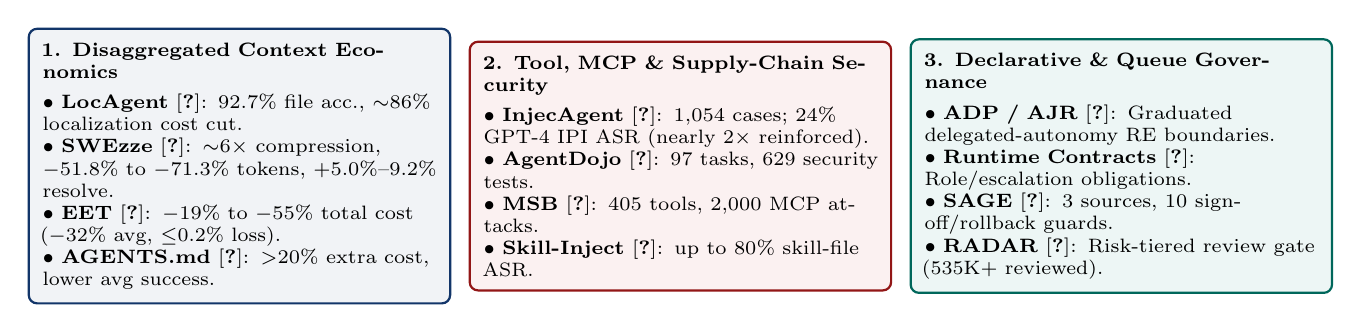
\begin{tikzpicture}[
    gbox/.style={rectangle, rounded corners=3pt, draw=navyblue, thick, fill=softgray, text width=5.0cm, minimum height=2.3cm, align=left, font=\scriptsize, inner sep=5pt}
]
\node[gbox, fill=navyblue!6] (c1) at (0,0) {
\textbf{1. Disaggregated Context Economics}\\[3pt]
$\bullet$ \textbf{LocAgent}~\cite{chen2025locagent}: 92.7\% file acc., $\sim$86\% localization cost cut.\\
$\bullet$ \textbf{SWEzze}~\cite{jia2026compressing}: $\sim$6$\times$ compression, $-$51.8\% to $-$71.3\% tokens, +5.0\%--9.2\% resolve.\\
$\bullet$ \textbf{EET}~\cite{guo2026eet}: $-$19\% to $-$55\% total cost ($-$32\% avg, $\le$0.2\% loss).\\
$\bullet$ \textbf{AGENTS.md}~\cite{gloaguen2026evaluating}: $>$20\% extra cost, lower avg success.};

\node[gbox, fill=crimson!6, draw=crimson!80!black] (c2) at (5.6,0) {
\textbf{2. Tool, MCP \& Supply-Chain Security}\\[3pt]
$\bullet$ \textbf{InjecAgent}~\cite{zhan2024injecagent}: 1,054 cases; 24\% GPT-4 IPI ASR (nearly 2$\times$ reinforced).\\
$\bullet$ \textbf{AgentDojo}~\cite{andriushchenko2024agentdojo}: 97 tasks, 629 security tests.\\
$\bullet$ \textbf{MSB}~\cite{zhang2025mcp}: 405 tools, 2,000 MCP attacks.\\
$\bullet$ \textbf{Skill-Inject}~\cite{schmotz2026skillinject}: up to 80\% skill-file ASR.};

\node[gbox, fill=tealaccent!7, draw=tealaccent!85!black] (c3) at (11.2,0) {
\textbf{3. Declarative \& Queue Governance}\\[3pt]
$\bullet$ \textbf{ADP / AJR}~\cite{arora2026specifying}: Graduated delegated-autonomy RE boundaries.\\
$\bullet$ \textbf{Runtime Contracts}~\cite{ciancarini2026charge}: Role/escalation obligations.\\
$\bullet$ \textbf{SAGE}~\cite{feng2026sage}: 3 sources, 10 sign-off/rollback guards.\\
$\bullet$ \textbf{RADAR}~\cite{adams2026automating}: Risk-tiered review gate (535K+ reviewed).};
\end{tikzpicture}
\caption{Three-Pillar Governance Architecture Synthesized from RQ4: Disaggregated Context Efficiency, Tool/MCP Containment, and Contract/Queue Controls.}
\label{fig:governance}
\end{figure*}

\textbf{1) Disaggregated Context Retrieval, Distillation, and Trajectory Economics.} Results across \textbf{57 primary \texttt{RQ4} studies} (103 multi-label \texttt{RQ4}-tagged studies) indicate that unselective context concatenation hurts long-horizon reasoning while driving up token spend~\cite{liu2024lost,kapoor2024agents}. For example, Gloaguen et al.~\cite{gloaguen2026evaluating} find that static repository overview files (\texttt{AGENTS.md}) slightly \emph{lower} average task success while adding \textbf{over 20\%} to inference cost. Separating cost-control methods by stack layer (Figure~\ref{fig:governance}) highlights three complementary levers: (i) in \emph{localization}, Chen et al.~\cite{chen2025locagent} report with \texttt{LocAgent} that indexing repositories as heterogeneous entity graphs reaches \textbf{92.7\%} file-level localization accuracy with a fine-tuned 32B open model at \textbf{$\sim$86\% lower localization cost} than proprietary baselines (+12\% Pass@10 issue resolution), alongside \texttt{RepoGraph}~\cite{ouyang2025repograph}, \texttt{CodexGraph}~\cite{liu2025codexgraph}, \texttt{RepoCoder}~\cite{zhang2023repocoder}, \texttt{CodeRAG-Bench}~\cite{wang2025coderagbench}, \texttt{CoRNStack}~\cite{suresh2025cornstack}, and \texttt{RepoNav}~\cite{chai2026reponav}; (ii) in \emph{prompt compression}, Jia et al.~\cite{jia2026compressing} show with \texttt{SWEzze} that distilling compact task-relevant contexts ($\sim$6$\times$ compression) cuts token budgets by \textbf{51.8\%--71.3\%} while improving SWE-bench Verified resolution by 5.0\%--9.2\%; and (iii) in \emph{trajectory control}, Guo et al.~\cite{guo2026eet} report that experience-driven early termination (\texttt{EET}) lowers total agent cost by \textbf{19\%--55\%} (\textbf{32\% average}) with at most 0.2\% resolution loss.

\textbf{2) Indirect Prompt Injection, MCP Connectors, and Skill Supply Chains.} Giving coding agents shell access, web search, and external tool connectors widens their security surface~\cite{pearce2023examining,greshake2023not}. On \texttt{InjecAgent} (1,054 cases across 17 user and 62 attacker tools), Zhan et al.~\cite{zhan2024injecagent} observe a \textbf{24\%} attack success rate on ReAct-prompted GPT-4 (nearly doubling under reinforced prompts), motivating stateful evaluation in \texttt{AgentDojo} (97 tasks, 629 security tests)~\cite{andriushchenko2024agentdojo} as well as defenses like \texttt{Task Shield}~\cite{jia2024task} and tool-dependency-graph \texttt{IPIGuard}~\cite{an2025ipiguard}. Recent studies also examine supply-chain risks in tool protocols and skill packages: on \texttt{MCP Security Bench} (405 tools, 2,000 attacks across 9 agents), Zhang et al.~\cite{zhang2025mcp} report that models with stronger instruction following can be \emph{more} susceptible to poisoned MCP tool metadata, and on \texttt{Skill-Inject} (202 skill-file pairs), Schmotz et al.~\cite{schmotz2026skillinject} measure up to an \textbf{80\%} attack success rate on frontier models, including data exfiltration and destructive commands.

\textbf{3) Requirements Delegation and Runtime Coordination Contracts.} Recent 2026 governance studies treat delegation boundaries as explicit engineering artifacts before code is written or merged. Arora et al.~\cite{arora2026specifying} propose \emph{Agency Justification Records} (AJRs) and tiered \emph{Agentic Delegation Policies} (ADPs) defining autonomy tiers, human oversight, and fallback rules; Ciancarini~\cite{ciancarini2026charge} specifies \emph{runtime coordination contracts} covering role scopes, I/O schemas, and escalation triggers; and Feng et al.~\cite{feng2026sage} introduce \texttt{SAGE}, coordinating multi-agent requirements clarification via three co-evolving sources and ten declarative transition guards for sign-off and rollback traceability (while noting that their evaluation demonstrates constraint encodability and traceability rather than field causal impact).

\section{Benchmark Design, Sensitivity Analysis, and Roadmap}
\label{sec:discussion}

\begin{table*}[t!]
\centering
\caption{Overview of 16 Representative Agentic SE Benchmarks and Telemetry Datasets.}
\label{tab:benchmarks}
\scriptsize
\setlength{\tabcolsep}{3.6pt}
\begin{tabularx}{\textwidth}{>{\raggedright\arraybackslash}p{2.15cm} >{\raggedright\arraybackslash}p{2.65cm} >{\raggedright\arraybackslash}p{2.55cm} X}
\toprule
\textbf{Benchmark / Dataset} & \textbf{Citation} & \textbf{Scale \& Scope} & \textbf{Primary Evaluation Focus \& Methodological Considerations} \\
\midrule
SWE-bench & Jimenez et al.~\cite{jimenez2024swebench} & 2,294 issues (12 Python repos) & Foundational real-world repo-repair benchmark; catalyzed subsequent leakage and test-strength refinements. \\
SWE-Bench+ & Aleithan et al.~\cite{aleithan2026swebench} & Leakage-filtered SWE-bench & Quantifies 32.67\% issue-comment leakage \& 31.08\% weak-test passes (12.47\% $\rightarrow$ 3.97\%). \\
UTBoost & Yu et al.~\cite{yu2025utboost} & Augmented Python test suites & Automated test augmentation identifying 345 under-tested patches; updates 40.9\% Lite \& 24.4\% Verified ranks. \\
SWT-Bench & M\"undler-Sasahara et al.~\cite{mndlersasahara2024swtbench} & Issue-to-test generation & Evaluates bug-reproducing test synthesis; doubles SWE-agent patch precision as filter. \\
Multi-SWE-bench & Zan et al.~\cite{zan2025multiswebench} & 1,632 tasks (7 languages) & Extends issue resolution to Java, TS, JS, Go, Rust, C, C++ (68 expert annotators). \\
SWE-smith & Yang et al.~\cite{yang2025swesmith} & 50k instances (128 repos) & Automated synthetic bug-breaking environments; trains 32B open model to 40.2\% Verified. \\
SWE-Gym & Pan et al.~\cite{pan2025training} & 2,438 executable Python tasks & Executable RL/verifier training environment yielding +19\% absolute resolve gains. \\
LiveCodeBench & Jain et al.~\cite{jain2025livecodebench} & 400 contest tasks (3 platforms) & Contamination-free rolling benchmark for generation, self-repair, execution, and test prediction. \\
ChainSWE & Jin et al.~\cite{jin2026chainswe} & 304 chained issues (54 projects) & Evaluates sequential maintenance chains; documents up to 70\% multi-issue performance drop. \\
FeatureBench & Zhou et al.~\cite{zhou2026featurebench} & 200 features (3,825 envs) & Multi-PR feature synthesis; 74.4\% SWE-bench model reaches 11.0\% on end-to-end features. \\
MCR-Bench & Zheng et al.~\cite{zheng2026static} & 2,269 multi-round reviews (5 langs) & Tracks defect lifecycle state across multi-round reviews, highlighting multi-turn tracking challenges. \\
SecLLMHolmes & Ullah et al.~\cite{ullah2024llms} & 228 security code scenarios & Evaluates vulnerability reasoning; identifier renaming or library edits alter 17\%--26\% of verdicts. \\
AIDev & Li et al.~\cite{li2026aidev} & 932,791 Agentic-PRs (116,211 repos) & Ecosystem-scale telemetry across 5 coding agents (33,596 curated PRs in 2,807 $>$100-star repos). \\
InjecAgent & Zhan et al.~\cite{zhan2024injecagent} & 1,054 IPI cases (17 user, 62 attacker tools) & Benchmarks indirect prompt injection exfiltration/harm across 30 tool-integrated agents. \\
AgentDojo & Andriushchenko et al.~\cite{andriushchenko2024agentdojo} & 97 tasks / 629 security tests & Dynamic stateful environment for adaptive prompt injection attacks and defenses. \\
MCP Security Bench & Zhang et al.~\cite{zhang2025mcp} & 405 MCP tools / 2,000 attacks & End-to-end 12-attack MCP harness showing higher susceptibility in stronger instruction-following models. \\
\bottomrule
\end{tabularx}
\end{table*}
\begin{table*}[t!]
\centering
\caption{Publication-Stage Sensitivity Check: Full Corpus ($N = 193$) vs.\ Formally Published Subset ($n = 155$, 80.3\%). Every citation in Column 3 is programmatically verified to satisfy \texttt{peer\_reviewed == True} in \texttt{review\_matrix.csv}.}
\label{tab:sensitivity}
\scriptsize
\setlength{\tabcolsep}{3.8pt}
\begin{tabularx}{\textwidth}{>{\raggedright\arraybackslash}p{2.75cm} X X >{\raggedright\arraybackslash}p{2.45cm}}
\toprule
\textbf{Thematic Pillar} & \textbf{Full Corpus Synthesis ($N = 193$)} & \textbf{Formally Published Subset ($n = 155$)} & \textbf{Sensitivity Verdict} \\
\midrule
RQ1: Code-supply surge vs. review-queue bottleneck & Enterprise RCTs report +26.08\% task throughput, whereas OSS developer RCTs (+19\% time) and PR telemetry (+105.9\% YoY LoC/diff reported at Meta; 3.5x merge delay under PR-MCI; 45.1\% of n=567 Claude PRs revised; -23.17 pp CRA-only merge rate) highlight downstream review load.~\cite{cui2026effects,becker2025measuring,adams2026automating,gong2026analyzing,watanabe2025use,oukhay2026code,chowdhury2026industry} & Consistent across N=4,867 enterprise RCTs (+26.08\% tasks), published Meta telemetry (535K+ reviewed / 331K+ landed diffs), high-MCI PR delays (3.5x merge time across 23,247 PRs), Claude PR edits (45.1\%, n=567), MSR reverts (2.66\%), and CRA merge gaps (-23.17 pp).~\cite{cui2026effects,adams2026automating,gong2026analyzing,watanabe2025use,oukhay2026code,chowdhury2026industry} & Directionally consistent (High confidence) \\
RQ1: Multi-agent coordination overhead vs. minimalist pipelines & Open-ended multi-agent ensembles exhibit 14 recurring misalignment/verification failure modes (MAST), while structured 3-stage pipelines (Agentless: 32.00\% at \$0.70) and sequential/feature benchmarks report up to 70\% multi-bug decay (ChainSWE) and 74.4\%->11.0\% feature drop (FeatureBench).~\cite{cemri2025multiagent,xia2024demystifying,jin2026chainswe,zhou2026featurebench} & Consistent across NeurIPS, FSE, and ACL/EMNLP studies: MAST (1,600+ traces, kappa=0.88), Agentless (\$0.70/issue), and ChainSWE (up to 70\% sequential maintenance drop across 304 chained issues).~\cite{cemri2025multiagent,xia2024demystifying,jin2026chainswe} & Directionally consistent (High confidence) \\
RQ2: Patch-overfitting \& benchmark oracle inflation & Static test suites overestimate repair accuracy via 32.67\% solution leakage \& 31.08\% weak tests, 345 under-tested passed patches (UTBoost), +6.4 pp behavioral divergence (PatchDiff), assertion-editing shortcuts (ImpossibleBench), and 73\%->43\% semantic gap reported at Google.~\cite{aleithan2026swebench,yu2025utboost,wang2025solved,rondon2025evaluating,mndlersasahara2024swtbench,zhong2025impossiblebench} & Consistent across AIware, ACL, NeurIPS, and ICSE studies: 12.47\%->3.97\% leakage/weak-test filtered resolve rate, 40.9\% Lite / 24.4\% Verified rank shifts, +6.4 pp PatchDiff inflation, SWT-Bench precision doubling, and Google Passerine gap (73\%/25.6\% vs. 43\%/17.9\%).~\cite{aleithan2026swebench,yu2025utboost,wang2025solved,rondon2025evaluating,mndlersasahara2024swtbench} & Directionally consistent (High confidence) \\
RQ3: Neuro-symbolic AST/PDG \& formal verification gains & All 15 primary L3.1 studies are formally published: coupling LLMs with AST/SBFL search, dataflow SMT solvers, execution alignment, and model checking yields substantial gains (VERT 1\%->42\%; LLMDFA 87.10\% precision; TransAgent +33.3\% accuracy; Syzygy C-to-safe-Rust).~\cite{zhang2024autocoderover,wang2024llmdfa,yang2024vert,shetty2025syzygy,yuan2024transagent,pan2024lost} & Identical across all 15 L3.1 primary studies (ISSTA, NeurIPS, OOPSLA, FSE, ICSE): AutoCodeRover (\$0.43 AST/SBFL), LLMDFA (87.10\% precision), VERT (1\%->42\% model checking), TransAgent (+56.7\% repair), Lost in Translation (1,700 samples), and Syzygy.~\cite{zhang2024autocoderover,wang2024llmdfa,yang2024vert,shetty2025syzygy,yuan2024transagent,pan2024lost} & Identical subset (High confidence) \\
RQ4: Disaggregated context savings, MCP risk \& governance & Graph localization cuts localization cost \textasciitilde{}86\% (LocAgent), distillation cuts token budget 51.8\%-71.3\% (SWEzze), and early stopping cuts total cost 19\%-55\% / 32\% avg (EET), whereas static AGENTS.md adds >20\% cost; IPI/MCP/skill channels reach 24\%-80\% ASR.~\cite{chen2025locagent,jia2026compressing,guo2026eet,gloaguen2026evaluating,zhan2024injecagent,zhang2025mcp,schmotz2026skillinject,arora2026specifying,feng2026sage} & Core cost \& IPI findings hold across ACL, ASE, NeurIPS, ICSE, and JLAMP studies: LocAgent (\textasciitilde{}86\% localization cost cut), SWEzze (-51.8\% to -71.3\% token budget), EET (-19\% to -55\% / -32\% avg total cost), InjecAgent/AgentDojo IPI defenses, and ADP/SAGE governance.~\cite{chen2025locagent,jia2026compressing,guo2026eet,zhan2024injecagent,andriushchenko2024agentdojo,arora2026specifying,ciancarini2026charge,feng2026sage} & Core consistent; MCP/AGENTS.md metrics extended by recent preprints \\
\bottomrule
\end{tabularx}
\end{table*}

\begin{table*}[t!]
\centering
\caption{Deterministic Five-Criterion Quality and Risk-of-Bias (RoB) Scoring Rubric (0--2 Points per Dimension; Total Score 0--10).}
\label{tab:rob_rubric}
\scriptsize
\setlength{\tabcolsep}{3.8pt}
\begin{tabularx}{\textwidth}{l >{\raggedright\arraybackslash}p{2.55cm} X X X}
\toprule
\textbf{ID} & \textbf{Dimension} & \textbf{Score 2} & \textbf{Score 1} & \textbf{Score 0} \\
\midrule
\texttt{Q1} & Publication Stage & Peer-reviewed journal or main conference proceedings article ($n=150$). & Refereed companion industry track or PC-reviewed workshop paper ($n=5$). & Moderated preprint not yet formally published in archival proceedings ($n=38$). \\
\texttt{Q2} & Empirical Design \& Control & RCT, multi-baseline benchmark ablation, or formal solver/model-checking proof. & Observational repository cohort or single-baseline empirical study. & Conceptual governance framework or qualitative case study without quantitative ablation. \\
\texttt{Q3} & Benchmark \& Cohort Scale & Multi-repository benchmark ($\ge 100$ tasks) or large field/PR cohort ($\ge 500$ PRs/devs). & Bounded repository evaluation, single-language suite, or medium developer sample. & Small illustrative case study or narrow synthetic micro-task evaluation. \\
\texttt{Q4} & Artifact \& Reproducibility & Publicly archived code, prompts/harnesses, and verifiable dataset identifiers. & Partial replication scripts, dataset metadata, or public benchmark leaderboard logs. & Proprietary internal telemetry or closed pipeline without public code release. \\
\texttt{Q5} & Oracle \& Contamination Control & Explicit contamination audit, differential/mutation oracle, or human semantic check. & Standard execution test suite with clear temporal window or baseline controls. & Unaudited static pass rate or unmitigated benchmark overlap risk. \\
\bottomrule
\end{tabularx}
\end{table*}

\subsection{Design Trade-Offs in Evaluation Benchmarks}
Table~\ref{tab:benchmarks} compares 16 representative benchmark and telemetry suites in our corpus. Across generations of benchmarks, three design trade-offs stand out: (i) \emph{single-issue repository resets}, where resetting to a clean snapshot after each fix isolates per-bug performance but hides cumulative drift addressed by sequential and multi-commit suites (\texttt{ChainSWE}~\cite{jin2026chainswe}, \texttt{FeatureBench}~\cite{zhou2026featurebench}); (ii) \emph{test-oracle completeness}, motivating leakage filtering (\texttt{SWE-Bench+}~\cite{aleithan2026swebench}), differential patch testing (\texttt{PatchDiff}~\cite{wang2025solved}), and automated test augmentation (\texttt{UTBoost}~\cite{yu2025utboost}); and (iii) \emph{unbounded inference budgets}, where leaderboards without token or dollar caps obscure cost--accuracy trade-offs~\cite{kapoor2024agents}.

\subsection{Risk-of-Bias Profile, Publication Bias, and Publication-Stage Sensitivity}
Across our 5-criterion Quality/RoB rubric in Table~\ref{tab:rob_rubric} (\texttt{03\_\allowbreak extraction/\allowbreak quality\_\allowbreak rob\_\allowbreak assessment.\allowbreak csv}), \textbf{Low RoB} corresponds to scores 8--10 ($n=132$), \textbf{Moderate RoB} to scores 5--7 ($n=56$), and \textbf{Elevated RoB} to scores $\le 4$ ($n=5$). Dimension \texttt{Q1} objectively records publication stage as of the search cutoff rather than intrinsic research quality (many widely cited preprints achieve Low RoB scores of 8/10), while deductions in \texttt{Q2}/\texttt{Q3} reflect conceptual or observational designs without controlled baselines or multi-repository samples. The 5 Elevated RoB studies~\cite{shetty2025syzygy,wen2025hammer,he2026attriguard,arora2026specifying,kanvar2026meets} each scored 4/10 due to bounded task scope or conceptual/case-study focus without quantitative ablations (itemized in Appendix~\ref{app:rubric}), and no headline quantitative conclusion in this review rests solely on Elevated RoB studies. While positive-result reporting in system papers can overstate agent capability, 2025--2026 replication and oracle studies~\cite{aleithan2026swebench,yu2025utboost,wang2025solved,ullah2024llms} alongside large-scale PR mining~\cite{gong2026analyzing,oukhay2026code,chowdhury2026industry} provide balancing empirical evidence. As a routine methodological check, Table~\ref{tab:sensitivity} compares all five thematic findings across the full corpus ($N=193$) and the \textbf{$n = 155$ formally published subset (80.3\%)}. Every main finding---the gap between bounded task speedups and downstream review friction~\cite{cui2026effects,adams2026automating,watanabe2025use,gong2026analyzing,oukhay2026code,chowdhury2026industry}, multi-agent coordination overhead and multi-step decay~\cite{cemri2025multiagent,xia2024demystifying,jin2026chainswe}, static test-suite overestimation~\cite{aleithan2026swebench,yu2025utboost,wang2025solved,rondon2025evaluating}, neuro-symbolic verification gains~\cite{zhang2024autocoderover,wang2024llmdfa,yang2024vert,shetty2025syzygy,pan2024lost}, and layered context compression with contract governance~\cite{chen2025locagent,jia2026compressing,guo2026eet,zhan2024injecagent,arora2026specifying,feng2026sage}---holds in the same direction, while recent preprints extend empirical coverage to OSS maintainer RCTs~\cite{becker2025measuring}, multi-PR feature tasks~\cite{zhou2026featurebench}, static \texttt{AGENTS.md} overhead~\cite{gloaguen2026evaluating}, and MCP/skill security~\cite{zhang2025mcp,schmotz2026skillinject}.

We also note the temporal cutoff effect of our age-stratified citation threshold \texttt{G4} ($\ge 18$ citations for 2026 preprints as of \texttt{2026-11-11}). While \texttt{G4} keeps our quantitative synthesis anchored in peer-reviewed or broadly cited studies, preprints posted in September--October 2026 had only 2--8 weeks to accrue citations and were therefore filtered under \texttt{EC5} unless already accepted at a peer-reviewed venue. As recorded in \texttt{03\_\allowbreak extraction/\allowbreak preprint\_\allowbreak quality\_\allowbreak gate\_\allowbreak audit.\allowbreak csv} (PRISMA Item \texttt{16b}), recent October 2026 preprints excluded solely by citation recency include \texttt{TestSuiteBench} (\texttt{arXiv:2610.13065}), \texttt{CRBugBench} (\texttt{arXiv:2610.13668}), and practitioner studies of reviewability and comprehension debt (\texttt{arXiv:2610.11179}), all of which align with the verification and review-queue findings observed across the included corpus.

\subsection{Seven-Challenge Research Roadmap}
Based on the synthesis above, we highlight seven research directions for agentic SE: (\textbf{C1}) \emph{Differential- and Coverage-Gated Benchmarks} complementing unit-test pass rates with PatchDiff~\cite{wang2025solved}, UTBoost~\cite{yu2025utboost}, and execution-filtered test generation~\cite{alshahwan2024automated}; (\textbf{C2}) \emph{Empirically Calibrated Queue-Aware Review Routing} estimating $G/G/k$ queue parameters ($c_a^2, c_s^2, \rho$) from industrial PR logs and pairing Meta-style \texttt{RADAR} risk scoring~\cite{adams2026automating} with message--code consistency checks~\cite{gong2026analyzing}; (\textbf{C3}) \emph{Incremental Neuro-Symbolic Compilation Loops} integrating SMT dataflow~\cite{wang2024llmdfa} and bounded model checking~\cite{yang2024vert} into edit actions; (\textbf{C4}) \emph{Multi-Commit Architectural State Retention} addressing sequential and feature-level horizon decay~\cite{jin2026chainswe,zhou2026featurebench}; (\textbf{C5}) \emph{Oracle-Guided Context Distillation \& Early Stopping} favoring learned context distillation and early stopping~\cite{jia2026compressing,guo2026eet} over static \texttt{AGENTS.md} prompts~\cite{gloaguen2026evaluating}; (\textbf{C6}) \emph{Capability-Scoped MCP \& Skill Sandboxes} enforcing least-privilege dataflow over untrusted tool outputs~\cite{zhan2024injecagent,andriushchenko2024agentdojo,zhang2025mcp,schmotz2026skillinject}; and (\textbf{C7}) \emph{Executable Delegation \& Sign-Off Contracts} embedding ADP~\cite{arora2026specifying} and SAGE~\cite{feng2026sage} guards into CI/CD workflows.

\section{Threats to Validity}
\label{sec:threats}

\textbf{Construct Validity.} Defining ``agentic'' SE boundaries can blur single-turn autocomplete with multi-step tool loops, and Eq.~\eqref{eq:kingman} is an uncalibrated analytical model rather than a structurally estimated equation. We addressed this by separating closed-loop agent architectures (\texttt{IC1-A}) from workflow/RCT studies (\texttt{IC1-B}) in \texttt{00\_protocol.md}, reporting autocomplete RCTs~\cite{cui2026effects,peng2023impact} separately from repository-level agentic PR cohorts~\cite{watanabe2025use,gong2026analyzing,li2026aidev,adams2026automating}, and listing empirical $G/G/k$ calibration as an open problem (\texttt{C2}).

\textbf{Internal Validity.} Five internal validity limitations warrant discussion: (i) \emph{single-author screening and RoB scoring without dual-coder $\kappa$}, addressed through deterministic screening scripts (\texttt{stage2\_\allowbreak and\_\allowbreak 3\_\allowbreak prisma.\allowbreak py}), full candidate logs (\texttt{screening\_log.csv}), 25/25 landmark recall, and a 12-day blind 10\% ($n=20$) intra-rater check (\texttt{intra\_\allowbreak rater\_\allowbreak blind\_\allowbreak check\_\allowbreak n20.\allowbreak csv}) reaching 100.0\% agreement on inclusion/\texttt{primary\_rq} and 95.0\% on \texttt{rqs}; (ii) \emph{local protocol freeze rather than external registry deposit}, addressed via SHA-256-checksummed raw API payloads; (iii) \emph{abstract-scoped quote verification}, checking our 38-row ledger against primary abstracts rather than unparsed PDF tables; (iv) \emph{English-only filtering} (\texttt{IC4}), which may miss non-English industrial reports; and (v) \emph{observational confounding in OSS PR studies}~\cite{gong2026analyzing,oukhay2026code,watanabe2025use}, where non-random task selection and the absence of matched human-revert baselines limit causal inference.

\textbf{External \& Conclusion Validity.} Open-source Python benchmarks (\texttt{SWE-bench}) remain heavily represented relative to proprietary polyglot codebases, though 2025--2026 studies increasingly examine Java/Rust/C++~\cite{zan2025multiswebench,horikawa2025agentic} and industrial deployments reported at Meta and Google~\cite{adams2026automating,rondon2025evaluating,alshahwan2024automated}. Finally, while our age-stratified citation criterion (\texttt{G4}) filters out very recent late-2026 uploads that have not yet accrued citations, our publication-stage sensitivity check ($n=155$, Table~\ref{tab:sensitivity}) indicates that all five headline conclusions remain consistent across publication stages.

\section{Conclusion}
\label{sec:conclusion}

Across $N = 193$ primary studies spanning the exact 48-month window from November 1, 2022 through October 31, 2026 (155 peer-reviewed articles and 38 moderated preprints), empirical evidence indicates that autonomous coding agents have matured into industrial-scale patch producers, yet end-to-end delivery remains governed by the \textbf{Productivity--Verification Paradox}. Converting raw code-generation velocity into reliable software engineering progress requires co-evolving agent orchestration with differential and coverage-grounded verification oracles, neuro-symbolic program analysis, disaggregated context compression, capability-isolated MCP sandboxes, and risk-calibrated socio-technical review governance.

\section*{Data Availability, Funding, and Institutional Disclaimer}
\textbf{Data and Replication Artifact Availability.} The complete replication package for \texttt{M01\_\allowbreak agentic\_\allowbreak se\_\allowbreak slr\_\allowbreak 20261111} is provided directly in the accompanying supplementary replication archive across five verifiable sub-packages: the locally frozen protocol \texttt{00\_protocol.md}; search protocol metadata and normalized records in \texttt{01\_harvest/}; the 4,205-record screening log, 25-seed recall audit, and 20-study blind intra-rater audit (\texttt{intra\_\allowbreak rater\_\allowbreak blind\_\allowbreak check\_\allowbreak n20.\allowbreak csv}) in \texttt{02\_screening/}; the 1,300-preprint screening audit, 193-study RoB and review matrices, and 38-claim verbatim ledger in \texttt{03\_extraction/}; the 27-item PRISMA checklist, SHA-256 manifest \texttt{artifact\_\allowbreak sha256\_\allowbreak manifest.\allowbreak json}, and audit certificate in \texttt{04\_manuscript/}; plus deterministic screening and verification scripts \texttt{stage1\_harvest.py}--\texttt{stage6\_verify\_all.py}.

\textbf{Funding, Competing Interests, and Institutional Disclaimer.} This research was conducted independently by the author during personal time outside the scope of official employment duties at the China National Association of Engineering Consultants (CNAEC) and received no external or institutional financial support. The author declares no competing financial or non-financial interests. Any views, findings, or conclusions expressed in this article are solely those of the author and do not represent the official positions or policies of CNAEC.

\appendix
\section{Verbatim Database Search Queries (2022-11-01 to 2026-10-31)}
\label{app:queries}

All four bibliographic APIs were queried programmatically on \texttt{2026-11-11} with exact date bounds \texttt{2022-11-01} to \texttt{2026-10-31} (persisted verbatim in \texttt{01\_\allowbreak harvest/\allowbreak search\_\allowbreak protocol.\allowbreak json}):
\begin{itemize}[leftmargin=*,nosep]
    \item \textbf{OpenAlex (\texttt{api.openalex.org/works}, 1,323 hits; \texttt{from\_\allowbreak publication\_\allowbreak date:\allowbreak 2022-11-01,\allowbreak to\_\allowbreak publication\_\allowbreak date:\allowbreak 2026-10-31}):} \par\vspace{1pt}{\fontsize{6.4}{7.4}\selectfont\ttfamily\raggedright ("coding agent" OR "coding agents" OR "code agent" OR "code agents" OR "software engineering agent" OR "software engineering agents" OR "SWE agent" OR "SWE agents" OR "agentic software engineering" OR "agentic coding" OR "code review agent" OR "code review agents" OR "SWE-bench" OR "agent-computer interface" OR "LLM agent" OR "LLM agents" OR "LLM-based agent" OR "LLM-based agents" OR "multi-agent" OR "autonomous program repair" OR "AI coding assistant" OR "GitHub Copilot") AND ("repository-level" OR "software repository" OR "pull request" OR "pull requests" OR "code review" OR "program repair" OR "issue resolution" OR "bug fixing" OR "fault localization" OR "test generation" OR "mutation testing" OR "unit test" OR "vulnerability repair" OR "code translation" OR "software modernization" OR "developer productivity" OR "time-to-merge" OR "prompt injection" OR "requirements clarification" OR "context retrieval") AND ("empirical" OR "benchmark" OR "benchmarking" OR "evaluation" OR "evaluating" OR "randomized controlled trial" OR "field experiment" OR "case study" OR "taxonomy" OR "ablation")\par}
    \item \textbf{arXiv (\texttt{export.\allowbreak arxiv.\allowbreak org/\allowbreak api/\allowbreak query}, 2,224 hits):} \par\vspace{1pt}{\fontsize{6.4}{7.4}\selectfont\ttfamily\raggedright (ti:"coding agent" OR abs:"coding agent" OR ti:"coding agents" OR abs:"coding agents" OR ti:"code agent" OR abs:"code agent" OR ti:"software engineering agent" OR abs:"software engineering agent" OR ti:"SWE agent" OR abs:"SWE agent" OR ti:"agentic software engineering" OR abs:"agentic software engineering" OR ti:"agentic coding" OR abs:"agentic coding" OR ti:"code review agent" OR abs:"code review agent" OR ti:"SWE bench" OR abs:"SWE bench" OR ti:"agent computer interface" OR abs:"agent computer interface" OR ti:"LLM agent" OR abs:"LLM agent" OR ti:"multi agent" OR abs:"multi agent" OR ti:"autonomous program repair" OR abs:"autonomous program repair") AND (ti:"repository" OR abs:"repository" OR ti:"pull request" OR abs:"pull request" OR ti:"code review" OR abs:"code review" OR ti:"program repair" OR abs:"program repair" OR ti:"issue resolution" OR abs:"issue resolution" OR ti:"fault localization" OR abs:"fault localization" OR ti:"test generation" OR abs:"test generation" OR ti:"mutation" OR abs:"mutation" OR ti:"vulnerability" OR abs:"vulnerability" OR ti:"code translation" OR abs:"code translation" OR ti:"developer productivity" OR abs:"developer productivity" OR ti:"prompt injection" OR abs:"prompt injection") AND (cat:cs.SE OR cat:cs.AI OR cat:cs.CL OR cat:cs.PL OR cat:cs.CR) AND submittedDate:[202211010000 TO 202610312359]\par}
    \item \textbf{Crossref (\texttt{api.crossref.org/works}, 1,200 hits; \texttt{type:\allowbreak journal-article,\allowbreak proceedings-article}, \texttt{from-pub-date:\allowbreak 2022-11-01,\allowbreak until-pub-date:\allowbreak 2026-10-31}):} Six verbatim \texttt{query.bibliographic} strings: \par\vspace{1pt}{\fontsize{6.4}{7.4}\selectfont\ttfamily\raggedright (1) "coding agent" "software engineering" benchmark evaluation; (2) "SWE-bench" OR "SWE agent" "program repair" repository; (3) "LLM agent" "code review" OR "pull request" OR "test generation" empirical; (4) "multi-agent" "code generation" OR "software development" benchmark evaluation; (5) "GitHub Copilot" OR "AI coding" "developer productivity" OR "pull request" empirical; (6) "coding agents" "mutation" OR "prompt injection" OR "requirements" software.\par}
    \item \textbf{Semantic Scholar (\texttt{api.\allowbreak semanticscholar.\allowbreak org/\allowbreak graph/\allowbreak v1/\allowbreak paper/\allowbreak search/\allowbreak bulk}, 1,299 hits; \texttt{fieldsOfStudy=\allowbreak Computer Science}, \texttt{publicationDateOrYear=\allowbreak 2022-11-01:\allowbreak 2026-10-31}):} \par\vspace{1pt}{\fontsize{6.4}{7.4}\selectfont\ttfamily\raggedright ("coding agent" | "coding agents" | "code agent" | "code agents" | "software engineering agent" | "software engineering agents" | "SWE agent" | "SWE agents" | "agentic software engineering" | "agentic coding" | "code review agent" | "code review agents" | "SWE-bench" | "agent-computer interface" | "LLM agent" | "LLM agents" | "LLM-based agent" | "LLM-based agents" | "multi-agent" | "autonomous program repair" | "AI coding assistant" | "GitHub Copilot") + ("repository-level" | "software repository" | "pull request" | "pull requests" | "code review" | "program repair" | "issue resolution" | "bug fixing" | "fault localization" | "test generation" | "mutation testing" | "unit test" | "vulnerability repair" | "code translation" | "software modernization" | "developer productivity" | "time-to-merge" | "prompt injection" | "requirements clarification" | "context retrieval") + ("empirical" | "benchmark" | "benchmarking" | "evaluation" | "evaluating" | "randomized controlled trial" | "field experiment" | "case study" | "taxonomy" | "ablation")\par}
    \item \textbf{API-Verified Snowballing (75 records):} Backward and forward reference tracking across 65 documented seed identifiers resolved individually via OpenAlex/Crossref/arXiv APIs (\texttt{01\_\allowbreak harvest/\allowbreak records\_\allowbreak snowball.\allowbreak jsonl}), alongside non-circular recall verification on 25 peer-reviewed 2023--2025 landmark seeds (\texttt{02\_\allowbreak screening/\allowbreak seed\_\allowbreak recall\_\allowbreak audit.\allowbreak json}).
\end{itemize}

\section{PRISMA 2020 Reporting Checklist Summary}
\label{app:prisma}
\setcounter{table}{0}
\renewcommand{\thetable}{B\arabic{table}}
\renewcommand{\theHtable}{B.\arabic{table}}

Table~\ref{tab:prisma_checklist} summarizes compliance with all 27 items of the PRISMA 2020 statement~\cite{page2021prisma} (full item-by-item mapping in \texttt{04\_\allowbreak manuscript/\allowbreak prisma\_\allowbreak 2020\_\allowbreak checklist.\allowbreak md}).

\begin{table}[t!]
\centering
\caption{Summary Mapping of PRISMA 2020 Checklist Items (Items 1--27).}
\label{tab:prisma_checklist}
\scriptsize
\setlength{\tabcolsep}{2.8pt}
\begin{tabularx}{\columnwidth}{l >{\raggedright\arraybackslash}p{2.12cm} X}
\toprule
\textbf{Items} & \textbf{PRISMA Domain} & \textbf{Manuscript Location / Artifact} \\
\midrule
1--2 & Title \& Structured Abstract & Title, Abstract ($\le 300$ words) \\
3--4 & Rationale \& RQ Objectives & \S\ref{sec:intro}, \S\ref{sec:methodology}, Table~\ref{tab:rqs} \\
5--7 & Eligibility, Sources \& Queries & \S\ref{sec:methodology}, Table~\ref{tab:criteria}, App.~\ref{app:queries} \\
8--10 & Selection, Extraction \& Data & \S\ref{sec:methodology}, App.~\ref{app:rubric}, \texttt{screening\_log.csv}, \texttt{review\_matrix.csv} \\
11, 14--15 & Study RoB, Bias \& Certainty & \S\ref{sec:methodology}, \S\ref{sec:discussion} (Table~\ref{tab:rob_rubric}), App.~\ref{app:rubric}, \texttt{quality\_\allowbreak rob\_\allowbreak assessment.\allowbreak csv} \\
12--13 & Effect Measures \& Synthesis & \S\ref{sec:methodology}, Table~\ref{tab:provenance}, Table~\ref{tab:sensitivity} \\
16--17 & PRISMA Flow \& Study Profiles & Fig.~\ref{fig:prisma}, \S\ref{sec:taxonomy}, Fig.~\ref{fig:taxonomy}, Table~\ref{tab:rep40} \\
18--22 & RoB Results \& RQ Syntheses & \S\ref{sec:taxonomy}--\S\ref{sec:discussion}, Figs.~\ref{fig:paradox}--\ref{fig:governance}, Tables~\ref{tab:rq1_topologies}--\ref{tab:rob_rubric} \\
23 & Evidence Interpretation \& Limits & \S\ref{sec:discussion}, \S\ref{sec:threats} \\
24--27 & Protocol, Funding, COI \& Data & \S\ref{sec:methodology}, \texttt{00\_protocol.md}, Data Availability \\
\bottomrule
\end{tabularx}
\end{table}

\section{Quantitative Verification Protocol and Archival Audit Notes}
\label{app:rubric}

Using the deterministic 0--2 point anchor rules in Table~\ref{tab:rob_rubric} (Section~\ref{sec:discussion}.2, adapted from Kitchenham and Charters~\cite{kitchenham2007guidelines,kitchenham2015evidence}), \texttt{stage2\_\allowbreak and\_\allowbreak 3\_\allowbreak prisma.\allowbreak py} scored all $N=193$ primary studies in \texttt{03\_\allowbreak extraction/\allowbreak quality\_\allowbreak rob\_\allowbreak assessment.\allowbreak csv}.

\noindent\textbf{Automated Quantitative Assertion \& Borderline Audit Notes:}
\begin{itemize}[leftmargin=*,nosep]
    \item \textbf{Numeric-Token \& Substring Verification (\S\ref{sec:methodology}.3):} In \texttt{stage3\_\allowbreak extract\_\allowbreak and\_\allowbreak verify.\allowbreak py}, each of the 38 claims in \texttt{03\_\allowbreak extraction/\allowbreak verified\_\allowbreak evidence\_\allowbreak ledger.\allowbreak csv} is verified by stripping model/metric version tokens (\texttt{GPT-4}, \texttt{Claude 3.5}, \texttt{Qwen-2.5-Coder-32B}, \texttt{Pass@k}) and queueing notation (\texttt{G/G/k}), extracting all integer, decimal, and percentage tokens via regex \texttt{\textbackslash b\textbackslash d+(?:\textbackslash .\textbackslash d+)?\%?\textbackslash b}, and asserting 100\% exact presence inside the contiguous verbatim abstract quote.
    \item \textbf{Archival Track Inventory \& Intra-Rater Adjudication (\S\ref{sec:methodology}.2):} Peer-reviewed VoR studies comprise 150 main-track papers---including 4 ACM AIware main-track articles (\texttt{S054}~\cite{aleithan2026swebench}, \texttt{S149}~\cite{ogenrwot2026agenticflict}, \texttt{S171}~\cite{chung2026collaborator}, \texttt{S181}~\cite{galster2026configuring})---and 5 refereed companion/workshop papers explicitly tagged \texttt{Peer-Reviewed Companion/\allowbreak Workshop} in \texttt{review\_matrix.csv}: FSE Companion Industry Track \texttt{S034}~\cite{alshahwan2024automated}, ICSE Companion \texttt{S038}~\cite{bouzenia2024repairagent}, ICSE LLM4Code Workshop \texttt{S057}~\cite{shetty2025syzygy}, AI for Software Modernization Workshop \texttt{S192}~\cite{kanvar2026meets}, and ASE MAS-GAIN Workshop \texttt{S193}~\cite{feng2026sage}. In the 12-day blind 10\% ($n=20$) intra-rater check (\texttt{02\_\allowbreak screening/\allowbreak intra\_\allowbreak rater\_\allowbreak blind\_\allowbreak check\_\allowbreak n20.\allowbreak csv}), the sole secondary-tag discrepancy concerned \texttt{S106}~\cite{guo2026eet} (primary \texttt{RQ4}); because \texttt{S106} evaluates inference-cost stopping without measuring PR merge latency, it retained \texttt{RQ4} only.
    \item \textbf{Elevated RoB Study Profiles (\S\ref{sec:discussion}.2):} Five studies scored $\le 4/10$: \texttt{S057}~\cite{shetty2025syzygy} ($4$: \texttt{Q1=\allowbreak 1,\allowbreak  Q2=\allowbreak 0,\allowbreak  Q3=\allowbreak 0,\allowbreak  Q4=\allowbreak 1,\allowbreak  Q5=\allowbreak 2}), \texttt{S098}~\cite{wen2025hammer} ($4$: \texttt{Q1=\allowbreak 0,\allowbreak  Q2=\allowbreak 1,\allowbreak  Q3=\allowbreak 0,\allowbreak  Q4=\allowbreak 2,\allowbreak  Q5=\allowbreak 1}), \texttt{S142}~\cite{he2026attriguard} ($4$: \texttt{Q1=\allowbreak 0,\allowbreak  Q2=\allowbreak 1,\allowbreak  Q3=\allowbreak 0,\allowbreak  Q4=\allowbreak 2,\allowbreak  Q5=\allowbreak 1}), \texttt{S184}~\cite{arora2026specifying} ($4$: \texttt{Q1=\allowbreak 2,\allowbreak  Q2=\allowbreak 0,\allowbreak  Q3=\allowbreak 0,\allowbreak  Q4=\allowbreak 1,\allowbreak  Q5=\allowbreak 1}), and \texttt{S192}~\cite{kanvar2026meets} ($4$: \texttt{Q1=\allowbreak 1,\allowbreak  Q2=\allowbreak 0,\allowbreak  Q3=\allowbreak 0,\allowbreak  Q4=\allowbreak 1,\allowbreak  Q5=\allowbreak 2}).
\end{itemize}

\FloatBarrier
\bibliographystyle{unsrt}
\bibliography{references}

\end{document}
